\documentclass[a4paper,12pt]{article}
\usepackage[T1]{fontenc}
\usepackage[utf8]{inputenc}
\usepackage[ngerman]{babel}
\usepackage[pdftex]{hyperref}
\usepackage{floatflt}
\usepackage{graphicx}
\usepackage{tabularx}
\usepackage{xcolor}
\usepackage{framed}
\usepackage{changes}
\usepackage{tikz}
\usepackage{capt-of}
\usepackage{diagbox}
\usetikzlibrary{arrows.meta}
\usepackage[thmmarks, thref]{ntheorem}
\usepackage{amsmath, amssymb}
%\usepackage[amsmath, thmmarks, thref]{ntheorem}
\usepackage{verbatim}
\usepackage{fancyhdr}
\usepackage[hang]{footmisc}
\renewcommand{\subsectionmark}[\thepage]{\markright{{#1}}}
\textheight220mm
\headheight 28pt
\textwidth160mm
\oddsidemargin0mm
\evensidemargin0mm
\topmargin0mm
\pagestyle{headings}
\fancyhead[R]{\sectionmark}
\newcommand{\F}{\mathbb F}
\newcommand{\f}{\mathbb f}
\newcommand{\K}{\mathbb K}
\newcommand{\R}{\mathcal R}
\newcommand{\N}{\mathbb N}
\newcommand{\Z}{\mathbb Z}
\newcommand{\Q}{\mathbb Q}
\newcommand{\A}{\mathcal A}
\newcommand{\C}{\mathcal C}
\newcommand{\D}{\mathcal D}
\newcommand{\X}{\mathcal X}
\newcommand{\Y}{\mathcal Y}
\newcommand{\xL}{\mathcal L}
\newcommand{\xP}{\mathcal P}
\newcounter{Hilfssatz}
\newcounter{Definition}
\newcounter{Beispiel}
\newcounter{Satz}
\newcounter{Algorithmus}



\setlength{\parindent}{0pt}
\makeatletter
  \@addtoreset{Definition}{subsection}
\makeatother
\newenvironment{Definition}{
\bigskip
        
        \setlength{\parindent}{0pt}
        \addtocounter{Definition}{1}
        \textbf{\textsf{Definition \thesubsection.\theDefinition}:}\\}{
        \nopagebreak
        \vspace{-1.0ex}
        \bigskip
        
}
\makeatletter
  \@addtoreset{Hilfssatz}{subsection}
\makeatother
\newenvironment{Hilfssatz}{
\medskip
        
        \setlength{\parindent}{0pt}
        \addtocounter{Hilfssatz}{1}
        \textbf{\textsf{Hilfssatz \thesubsection.\theHilfssatz}:}\\}{
        \nopagebreak
        \vspace{-1.0ex}
        \bigskip\\
}

\makeatletter
  \@addtoreset{Satz}{subsection}
\makeatother
\newenvironment{Satz}{
\medskip
        
        \setlength{\parindent}{0pt}
        \addtocounter{Satz}{1}
        \textbf{\textsf{Satz \thesubsection.\theSatz}:}\\}{
        \nopagebreak
        \vspace{-1.0ex}
        \bigskip\\
        
}

\makeatletter
  \@addtoreset{Beispiel}{subsection}
\makeatother
\newenvironment{Beispiel}{
\medskip
        
        \setlength{\parindent}{0pt}
        \addtocounter{Beispiel}{1}
        \textbf{\textsf{Beispiel \thesubsection.\theBeispiel}:}\\}{
        \nopagebreak
        \vspace{-1.0ex}
        \bigskip
        
}

\setlength{\parindent}{0pt}
\newenvironment{proof}{
%\bigskip
        \setlength{\parindent}{0pt}
        \textbf{Beweis:}\\}{
        \nopagebreak
        \vspace{-1.0ex}
        \begin{flushright}
             $\square$
        \end{flushright}
        \bigskip
        
}

\makeatletter
  \@addtoreset{Algorithmus}{subsection}
\makeatother
\newenvironment{Algorithmus}{
\medskip
        
        \setlength{\parindent}{0pt}
        \addtocounter{Algorithmus}{1}
        \textbf{\textsf{Algorithmus \thesubsection.\theAlgorithmus}:}}{
        \nopagebreak
        \vspace{-1.0ex}
        \bigskip
        
}

\usepackage{lastpage}% F\"ur die Verweise innerhalb des  Symbolverzeichnisses

\usepackage{nomencl} % Symbolverzeichnis
\let\symb\nomenclature %% Es genuegt \symb statt \nomenclature zu  schreiben
\setlength{\nomlabelwidth}{.25\hsize}
\renewcommand{\nomlabel}[1]{#1 \dotfill}
\setlength{\nomitemsep}{-\parsep}\renewcommand{\nomname}
{Symbolverzeichnis}

\setlength{\nomitemsep}{-\parsep}
\usepackage{array} %notwendig um neue Spaltentypen zu definieren
\newcolumntype{B}[1]{>{\centering\arraybackslash}m{#1}}
\makenomenclature

\newcommand{\CC}{C\nolinebreak\hspace{-.05em}\raisebox{.4ex}{\tiny\bf+}\nolinebreak\hspace{-.10em}\raisebox{.4ex}{\tiny\bf+}\;}
\begin{document}
\begin{titlepage}
\thispagestyle{empty} \enlargethispage{1.4in}

\begin{center}

\rule[1ex]{157.5mm}{0.5mm}

\LARGE\bf Hochschule für angewandte Wissenschaften Coburg\\

\vfill

\rm Institut für Informatik


\begin{figure}
	    \centering
				     
\includegraphics[width=0.5\textwidth]{Logo.png}
\end{figure}

\vfill

\Huge \bf Asymmetrische Zahlensysteme

\vfill

\Large Bachelorarbeit \\ [1ex] von \\ [1ex]
Michael Krasser

\vfill

Betreuer:  Prof.\,Dr.~Quirin~Meyer

\vfill

Coburg, \today

\rule[-1ex]{157.5mm}{0.5mm}

\vfill

\end{center}

\end{titlepage}

\newpage
\tableofcontents
\pagebreak
\section{Einleitung}
Im Zeitalter der Digitalisierung werden immer größere Datenmengen produziert, gespeichert und übertragen, was sowohl den Einsatz als auch die Suche nach effizienten Verfahren zur Datenkom{\tt{pre}}ssion unerläßlich macht.
Hierfür schlägt Jaroslaw Duda\cite{Duda} ein neues Verfahren mit dem Namen "`asymmetrische Zahlensysteme"' vor, das seitdem von Unternehmen wie Facebook\cite{fb}, Google\cite{google} und Apple\cite{apple} verwendet wird. 
Im Rahmen dieser Bachelorarbeit über asymmetrische Zahlensysteme sollen zunächst grundlegende Begriffe aus dem Bereich der Codierungstheorie geklärt und gänge Entropiecodierer besprochen werden.
Anschließend sollen die in \cite{Giesen}, \cite{Duda} und \cite{Krajcevski} angegebene Verfahren {\tt{uabs}} und {\tt{rans}} untersucht werden.
\par
Ziel dieser Arbeit ist Verallgemeinerung des {\tt{uabs}}-Verfahrens auf ein $n$-elementiges Symbolalphabet ({\tt{uans}}-Verfahren) und die Anwendung des  {\tt{uans}}- sowie des {\tt{rans}}-Verfahren auf Bilddateien. Zusätzlich soll der Einfluß einer vorgeschalteten Filterung -- die in Kapitel ~\ref{Filter} besprochen wird -- untersucht werden. Hierfür werden die verwendeten Filter und die beiden Verfahren in \CC implementiert. 
\par
\vspace{0.5cm}
Nachfolgende Abbildung veranschaulicht den Programmfluss:

\begin{center}
{\color{gray!50!blue}\rule{9cm}{0.1mm}}
\vspace{0.2cm}
\\
\begin{tabular}{c c}
initialer Zustand & schreiben beendet 
\\
{\tt{readImage}} & {\tt{writeImage}}
\\
$\downarrow$ & $\uparrow$ 
\\
{\tt{normalize}} & 
\\
$\downarrow$ & 
\\
{\tt{execute{\tt{pre}}condition}} & {\tt{execute{\tt{post}}condition}}
\\
$\downarrow$ & $\uparrow$ 
\\
{\tt{encode}} & {\tt{decode}}
\\
$\downarrow$ & $\uparrow$ 
\\
{\tt{writeBinaryFile}} & {\tt{readBinaryFile}}
\\
$\downarrow$ & $\uparrow$ 
\\
finaler Zustand & finaler Zustand
\end{tabular}
{\color{gray!50!red}\rule{9cm}{0.1mm}}
\vspace{0.5cm}
\captionof{figure}{Programmfluß der Implementierung}
\end{center}
In Leserichtung wird das Bild gelesen, vorkonditionert, normalisiert und 
anschließend komprimiert.
Die Dekomprimierung erfolgt in umgekehrter Leserichtung. 
\par
In Kapitel ~\ref{Kommandozeilenparameter} findet sich eine Anleitung zur Bedienung der \CC Implementierung.
\newpage
\section{Kompression und Dekompression}
Dieser Abschnitt orientiert sich an\cite{henne} sowie \cite{Lajmi} und klärt die wichtigsten Begriffe aus dem Bereich Datenkompression und stellt gängige Entropiecodierer vor.
\subsection{Grundlagen}
\begin{Definition}
Unter Datenkompression versteht man ein Paar $(\X,\Y)$ von Algorithmen - Datenkompressionschema genannt, mit folgenden Eigenschaften:

Der Algorithmus $\X \; \left(Kompression\right)$ konstruiert für die Eingabe $X$ eine Repräsentation $X_c$, die (möglichst) weniger Bits als $X$ benötig.
\par
Der Algorithmus  $\Y \; \left(Dekompression\right)$ generiert zu gegebenem $X_c$ die Rekonstruktion $Y$.
\par
 Ein Datenkompressionschema heißt verlustfrei, wenn $X = Y$, ansonsten verlustbehaftet.
\end{Definition}
Desweiteren definiert man zur Beurteilung der Qualität eines Komprimierungsschemas:
\begin{Definition}
Sei $\mu_c$ die Anzahl der Bits von $X_c$ und $\mu$ die Anzahl der Bits von $X$. Dann heißt der durch
$
\mu_c \slash \mu
$
definierte Ausdruck Kompressionsquotient\footnote{\footnotesize{1Der Kehrwert des Kompressionsquotienten wird auch Kompressionsfaktor genannt.}}.
\end{Definition}
\subsection{Über die Möglichkeit der Datenkompression}
 Vesteht man unter Datenkompression ein Verfahren, das eine bestimmte Repräsentation in eine andere überführt, die stets weniger Bits als die urspüngliche benötigt, dann zeigt ein einfaches Abzählargument, dass es ein solches Verfahren nicht geben kann. Diese Argumentation wird in Arbeiten zum Thema Kolmogorov-Komplexität als sog. Inkompressibilitätsargument bezeichnet und begründet, warum sich bestimmte Bitfolgen nicht komprimieren lassen: Die Kolmogorov-Komplexität einer Bitfolge $t$ ist definiert als die Länge des kürzesten "`Programms"', welches $t$ erzeugt\footnote{\footnotesize{Bei geeigneter Formalisierung des Begriffs
"`Programm"' ist die Kolmogorov-Komplexität bis auf eine additive Konstante wohldefiniert.\cite{Li} }}. Eine Bitfolge heißt unkomprimierbar, falls sie selbst ihre kürzeste Beschreibung ist.
Trotzdem funktioniert die Datenkompression in der Praxis hervorragend:
\begin{itemize}
	\item Einzelne Zeichen (Grundelemente des Alphabets) tauchen nicht mit der selben Wahrscheinlichkeit auf. $\Rightarrow$ 
verschlüssele wahrscheinlichere Zeichen mit weniger Bit als unwahrscheinlichere (Morse-Alphabet).
\item Blöcke von Zeichen lassen sich aufgrund der Abhängigkeiten aufeinander folgender Ereignisse geschickter gemeinsam als lose unabhängige Folge einzelner Zeichen verschlüsseln.  
\item Information ist nicht zufällig, sondern enthält  zahllose Regelmäßigkeiten.
\par
 Eine Grundstrategie von Kompressionsverfahren beruht darauf, solche Regeln zu entdecken (z.B. Wörterbuchtechniken).
\item  Für oder von Menschen erzeugte Information ist nicht zusammenhangslos. Vielfach ist es möglich, verschiedene Gattungen von Information zu unterscheiden: Sei z.B. bekannt, dass die vorliegende Bitfolge einen ASCII-Text der englischen Sprache darstellt, so muss ein anderes Kompressionsverfahren (auf Byte-Ebene) als wenn die Bitfolge die zeilenweise Darstellung eines Schwarz-Weiß-Bildes repräsentiert (starke Abhängigkeiten von Bit zu Bit, zeilen- und spaltenweise).
\item Oft kann auf eine exakte Rekonstruierbarkeit des Originals verzichtet werden, da gewisse Feinheiten vom menschlichen Auge oder Ohr nicht wahrgenommen werden:  Frequenzen von Audiodaten, die für das menschliche Ohr gedacht sind und nicht wahrgenommen werden, können, von vornherein vernachlässigt werden.
\end{itemize}
\subsection{Entropiekodierer}
\subsubsection{Die Entropie}
\begin{Definition}
Gegeben sei eine diskrete Quelle $Q$ mit den Symbolen $x_{1},\ldots,x_{N}$ und dazugehörigen Wahrscheinlichkeiten $p_1,\ldots,p_N$.
\par
Bezeichne $I(x_{i}) = -\text{log}_{2}(p_{i})$ den Informationsgehalt des Symbols $x_{i}$.
Die Entropie (mittlere Informationsgehalt) von $Q$ ist definiert durch
\begin{align*}
H(Q):=\sum_{i=1}^N p(x_{i})\cdot I(x_{i}) =- \sum_{i=1}^N p(x_{i}) \cdot \text{log}_2(p(x_{i})).
\end{align*}
Die Entropie von $Q$ heißt maximal, wenn $H(Q) = \text{log}_2(N)$.
 Diese maximale Entropie wird mit $H_{0}$ bezeichnet und heißt Entscheidungsgehalt.
\end{Definition}
\begin{Definition}
Entropiekodierung bezeichnet ein Verfahren, welches die Entropie einer Nachricht optimiert, d. h., der maximalen Entropie annähert.
\end{Definition}
Abschließend definieren wir den Begriff der  {\it Redundanz und der erwarteten Länge} eines Codes:
\begin{Definition}
Sei $\Sigma = \{a_{1},\ldots, a_{k}\}$ ein Alphabet mit zugehörigen Auftrittswahrscheinlichkeiten 
$$
\{P(a_{i})\,|\,i=1,\ldots,k\}.
$$
Die Kodierung $\mathcal{K}: \Sigma\rightarrow \{0, 1\}^{\N}$ besitzt die erwartete Länge
\begin{align*}
L(\mathcal{K}):=\sum_{i=1}^{k} P(a_{i})\cdot \left| \mathcal{K}(a_{i})\right|.
\end{align*}
Der Term 
\begin{align*}
r:=L(\mathcal{K}) - H(\Sigma)
\end{align*}
bezeichnet die Redundanz der Kodierung.
\end{Definition}
\subsubsection{Kom{\tt{pre}}ssion nach dem Verfahren von Shannon}
Nach Shannon gilt:
\begin{Satz}
Für Jede Quelle $Q$ und jede beliebige zugehörige Binärcodierung mit 
Präfix-Eigenschaft ist die zugehörige mittlere Codewortlänge $L$ 
nicht kleiner als die Entropie $H(Q)$: $H(Q)\leq L$
\end{Satz}
\begin{proof}
Siehe \cite{Rohling}.
\end{proof}
Um für einen gegebenen Text einen dekodierbaren Code mit minimaler Länge zu finden, geht man nach Shannon folgendermaßen vor:
\begin{itemize}
	\item[1)]  Sortiere zu kodierende Symbole $x_{1},\ldots,x_{N}$ nach fallender Auftrittswahrscheinlichkeit: 
$p_{1}\geq p_{2}\geq\ldots\geq p_{N}$.
	\item[2)] Bestimme für $1\leq i \leq N$ die Codewortlänge $\mathcal{K}(x_{i}) = \lfloor -\text{log}_2(p(x_{i}))\rfloor$ jedes Zeichens aus seinem Informationsgehalt.
	\item[3)] Berechne für $1\leq i \leq N$ die kumulierte Wahrscheinlichkeiten $P(x_{i}):=\sum_{l=0}^{i-1}p(x_{l})$.
	\item[4)] Die Codierung jedes Zeichens $x_{i}$ ergibt sich dann aus den ersten $\mathcal{K}(x_{i})$ Zeichen der Mantisse der Binärdarstellung von $P(x_{i})$.
\end{itemize}
\begin{Beispiel}

\begin{center}
\begin{tabular}{c|c|c|c|c|c}
$x_{i}$ & $p(x_{i})$ & $\mathcal{K}(x_{i})$ & $P(x_{i})$ & binär & Code
\\
\hline
a & 0.3 & 2 & 0 & $0.000\ldots$ & 00
\\
\hline
b & 0.3  & 2 & 0.3 & 0.0100\ldots & 01
\\
\hline
c & 0.2  & 3 & 0.6 & 0.1001\ldots & 100
\\
\hline
d & 0.1  & 4 & 0.8 & 0.1100\ldots & 1100
\\
\hline
e & 0.1  & 4 & 0.9 & 0.1110\ldots & 1110
\end{tabular}
\end{center}
\end{Beispiel}
Dieses Verfahren ist eines der ersten zur Erstellung von präfixfreien, längenvariablen Codes.
\subsubsection{Kom{\tt{pre}}ssion nach dem Verfahren von Fano}
Ein weiteres Beispiel für einen Präfixcode ist die Shannon-Fano Codierung:
\begin{itemize}
\item[1)] Sortiere zu kodierende Symbole $x_{1},\ldots,x_{N}$ nach fallender Auftrittswahrscheinlichkeit: 
$p_{1}\geq p_{2}\geq\ldots\geq p_{N}$
\item[2)] Teile Menge der Symbole in 2 Teilmengen mit möglichst gleicher Wahrscheinlichkeit.
\item[3)] Kodiere linke Teilmenge mit 0, die rechte mit 1
\item[4)] Sind entstandene Teilmengen nicht einelementig, gehe zu 2.
\end{itemize}
\begin{Beispiel}
\begin{minipage}[h]{.8\textwidth}
Gegeben sei das vierelementige Alphabet $\left\{A, B, C, D\right\}$ mit zugehörigen
\par
 Auftrittswahrscheinlichkeiten
 $p_A =0.4,\, p_B = 0.3,\, p_C = 0.2,\, p_D =0.1$. Man erhält $A=0,\,B=111,\,C=110,\,D=10$
\\
\vspace{0.2cm}
\end{minipage}
\hfill
 \begin{minipage}[h]{.2\textwidth}
\begin{flushright}
$\underbrace{A}_{0} \;\underbrace{D\; C\; B\;}_{1}$
\\
\quad$\underbrace{D}_{0}\;\underbrace{C\; B\;}_{1}$
\\
\quad\quad$\underbrace{C}_{0}\;\underbrace{B}_{1}$
\end{flushright}
\end{minipage}    
\end{Beispiel}
\subsubsection{Huffman-Algorithmus}
Um einen Code auch wieder eindeutig dekodieren zu können, muss er die Kraftsche Ungleichung erfüllen und zusätzlich noch präfixfrei sein, d. h. kein Codewort darf der Beginn eines anderen sein. (An andere Stelle setzen......)
Die Huffman-Kodierung ist eine Form der Entropiekodierung, die 1952 von David A. Huffman entwickelt und in \cite{Huffman} publiziert wurde.
Die Kodierung ist ein Präfix-Code (also ein Code mit kleinster erwarteter Länge), der einer festen Anzahl von Quellsymbolen Codewörter mit variabler Länge zuordnet.
\begin{Algorithmus} (Huffmann-Kodierung)
\\
 Sei $\A$ ein Symbolalphabet, $p_{x}=p(x)$ die relative Häufigkeit des Symbols $x \in \A$, $\C$ das Codealphabet (Zeichenvorrat der Codewörter)
 $m=| \C |$ die Mächtigkeit von $\C$.
\par
\textbf{Aufbau des Baumes}
\begin{itemize}
	\item[1)] Erstelle für $x \in \A$ einen Knoten mit zugehöriger Häufigkeit.
	\item Wiederhole folgende Schritte, bis nur noch ein Baum übrig ist:
	\begin{itemize}
		\item[i)] Wähle die $m$ Teilbäume mit der geringsten Häufigkeit in der Wurzel, bei mehreren Möglichkeiten die Teilbäume mit der geringsten Tiefe.
		\item[ii)]  Fasse diese Bäume zu einem neuen (Teil-)Baum zusammen.
		\item[iii)]  Notiere die Summe der Häufigkeiten in der Wurzel.
	\end{itemize} 
\end{itemize}
\textbf{Konstruktion des Codebuchs}
\begin{itemize}
	\item[1)] Ordne jedem Kind eines Knotens eindeutig ein Zeichen aus dem Codealphabet zu.
	\item[2)]  Lies für jedes Quellsymbol (Blatt im Baum) das Codewort aus: Beginne an der Wurzel des Baums. Die Codezeichen auf den Kanten des Pfades (in dieser Reihenfolge) ergeben das zugehörige Codewort.
\end{itemize}   
\end{Algorithmus}
\begin{Beispiel}
Die Nachricht {\it aababcabcd} soll auf Basis des Codealphabets $\C=\{0,1\}$ kodiert werden. Zunächst erhält man
\begin{align*}
 \A = \{a, b, c, d\}\quad \text{mit}\quad
\begin{tabular}{c|c|c|c|c}
X & a & b & c & d
\\
\hline
P(X) & 0.4 & 0.3 & 0.2 & 0.1
\\
\end{tabular} 
\end{align*}
\textbf{Konstruktion des Huffman-Baums:}
\begin{align*}
\begin{tikzpicture}
 \draw(0.0,-0.75)node[]{a}
		(0.75,-0.75)node[circle=0.3cm,fill = gray]{0.4}
		 (1.0,-1.0) -- (1.5,-1.5)
		(1.75,-1.75) node [circle=0.3cm,fill = gray]{0.3}
		(0.75,-1.75) node []{b}
		(2.0,-2.0) -- (2.5,-2.5);
		\draw[->, blue!50, very thick] (4.5,-2.75) to[bend left=20]
 (5.5,-2.75);
		\draw
		(2.75,-2.75) node [circle=0.3cm, fill=red]{0.2}
		(1.5,-2.75) node []{c}
			(3.0,-3.0) -- (3.5,-3.5)
			(3.75,-3.75) node [circle=0.3cm, fill=red]{0.1}
			(2.25,-3.75) node []{d}
			%Ende 1
	(5.0,-0.75)node[]{a}
	(5.75,-0.75) node [circle=0.3cm,fill = gray]{0.4}
  (6.0,-1.0) -- (6.5,-1.5)
	(6.0,-1.75)node[]{b}
	(6.75,-1.75) node [circle=0.3cm,fill = gray]{0.3}
(7.0,-2.0) -- (7.5,-2.5)
(7.75,-2.75) node [circle=0.3cm]{0.3}
		(7.75,-3.0) -- (7.25,-3.5)
		(7.0,-4.5)node[]{c}
		(7.0,-3.75) node [circle=0.3cm, fill=red]{0.2};
		\draw[->, blue!50, very thick] (8.5,-2.75) to[bend left=20]
 (9.5,-2.75);
		\draw
		(7.75,-3.0) -- (8.25,-3.5)
		(8.5,-4.5)node[]{d}
		(8.5,-3.75) node [circle=0.3cm, fill=red]{0.1}
		%Ende 2
	(10.75,-0.75) node []{1.0}
	(11.0,-1.0) -- (11.0,-5.0)
  (11.0,-1.0) -- (12.0,-2.0)
	(12.25,-2.25) node []{0.6}
	(12.25,-2.5) -- (12.25,-5.0)
	(12.5,-2.5) -- (13.5,-3.5)
	(13.75,-3.75) node []{0.3}
	(14.0,-4.0) -- (15.0,-5.0)
	(14.0,-4.0) -- (14.0,-5.0)
	(15.25,-5.25) node [circle=0.3cm, fill=red]{0.1}
	(15.25,-6.0)node[]{d}
	(14.0,-5.25) node [circle=0.3cm, fill=red]{0.2}
	(14.0,-6.0)node[]{c}
	(12.25,-5.25) node [circle=0.3cm, fill=red]{0.3}
	(12.25,-6.0)node[]{b}
	(10.75,-5.25) node [circle=0.3cm, fill=red]{0.4}
	(10.75,-6.0)node[]{a};
\end{tikzpicture}
\end{align*}
\textbf{Konstruktion des Codebuchs:}
Dazu versehen wir jeden linken Zweig mit einer $1$, jeden rechten mit einer $0$:
\par
\hspace{1.5cm}
\begin{minipage}[h]{.5\textwidth}
\begin{tabular}{c|c}
Symbol & Verschlüsselung
\\
\hline
a & 1
\\
\hline
b & 01
\\
\hline
c & 001
\\
\hline
d & 000
\end{tabular}
\vspace{3cm}
\end{minipage}
\hfill
 \begin{minipage}[h]{.5\textwidth}
\begin{flushright}
\begin{tikzpicture}
\draw
(0.75,-0.75) node []{1.0}
  (0.7,-2.5) node []{1}
	(1.0,-1.0) -- (1.0,-5.0)
	(1.8,-1.5) node []{0}
  (1.0,-1.0) -- (2.0,-2.0)
	(2.25,-2.25) node []{0.6}
	(1.9,-3.75) node []{1}
	(2.25,-2.5) -- (2.25,-5.0)
	(3.3,-3.0) node []{0}
	(2.5,-2.5) -- (3.5,-3.5)
	(3.75,-3.75) node []{0.3}
	(4.8,-4.5) node []{0}
	(4.0,-4.0) -- (5.0,-5.0)
	(3.7,-4.5) node []{1}
	(4.0,-4.0) -- (4.0,-5.0)
	(5.25,-5.25) node [circle=0.3cm, fill=red]{0.1}
	(5.25,-6.0)node[]{d}
	(4.0,-5.25) node [circle=0.3cm, fill=red]{0.2}
	(4.0,-6.0)node[]{c}
	(2.25,-5.25) node [circle=0.3cm, fill=red]{0.3}
	(2.25,-6.0)node[]{b}
	(0.75,-5.25) node [circle=0.3cm, fill=red]{0.4}
	(0.75,-6.0)node[]{a};
\end{tikzpicture}
\end{flushright}
\hspace{1.5cm} 
\end{minipage} 
Damit kodiert sich die Nachricht {\it a 	a 	b 	a 	b 	c 	a 	b 	c 	d} zu
$1\, 	1\, 	01\, 	1\, 	01\, 	001\, 	1\, 	01\, 	001\, 	000$.\footnote{\footnotesize{Bei der Dekodierung verfolgt man ausgehend von der Wurzel den ents{\tt{pre}}chende Pfad im Baum bis man an einem Blatt ankommt.}}   
In diesem Fall erhält man für die Entropie und die erwartete Länge:
\begin{align*}
H(Q) &=-\left(  0.4 * \text{log}_{2}(0.4)   +   0.3 * \text{log}_{2}(0.3) +  0.2 * \text{log}_{2}(0.2)\right.\\
     &\left.\quad +  0.1 * \text{log}_{2}(0.1)\right) = 1.84643934467
\\
L(\mathcal{K})&= 0.4 + 2\cdot 0.3 + 3* 0.3 = 1.9,
\end{align*}
d.h bei einer zu kodierenden Nachricht von 1000000 Symbolen sind etwa 28190 Symbole redundant.
\end{Beispiel}
\subsubsection{Erweiterte Huffman-Codierung}
Wir betrachten einführend folgendes Beispiel: Sei $\Sigma = \{a, b\}$ mit $p(a)=0.9,\,p(b)=0.1$. Dann liefert die Huffman-Kodierung
\begin{center}
\begin{tabular}{c|c|c}
 & p & Code
\\
\hline
a & 0.9 & 1
\\
\hline
b & 0.1 & 0
\end{tabular}
\end{center}
mit erwarteter Länge $1$ Bits / Symbol und Entropie $H(\Sigma)=0.47$. Die Redundanz $r=0.53$ beträgt also $113\%$ der Entropie, d.h das der Code nicht komprimiert ist.
Wir betrachten statt dessen das Alphabet
\begin{align*}
\Sigma^{2}:= \{aa,ab,ba,bb\}
\end{align*}
mit $p(aa)=\left(p(a)\right)^{2}$, $p(bb)=\left(p(b)\right)^{2}$ und $p(ab)= p(ba) =p(a)\cdot p(b)$. Die Huffman-Kodierung liefert dann
\par
\hspace{1.5cm}
\begin{minipage}[h]{.5\textwidth}
\begin{tabular}{c|c|c}
Symbol & p & Verschlüsselung
\\
\hline
aa & 0.81 & 1
\\
\hline
ab & 0.09 & 01
\\
\hline
ba & 0.09 & 001
\\
\hline
bb & 0.01 & 000
\end{tabular}
\\
$H(\Sigma^{2})= 0.937991187$ Bits / Symbol
\\
$L(\mathcal(K)) = 1.29$ Bits / Symbol
\end{minipage}
\hfill
 \begin{minipage}[h]{.5\textwidth}
\begin{flushright}
\begin{tikzpicture}
\draw
(0.75,-0.75) node []{1.0}
  (0.7,-2.5) node []{1}
	(1.0,-1.0) -- (1.0,-5.0)
	(1.8,-1.5) node []{0}
  (1.0,-1.0) -- (2.0,-2.0)
	(2.25,-2.25) node []{0.19}
	(1.9,-3.75) node []{1}
	(2.25,-2.5) -- (2.25,-5.0)
	(3.3,-3.0) node []{0}
	(2.5,-2.5) -- (3.5,-3.5)
	(3.75,-3.75) node []{0.1}
	(4.8,-4.5) node []{0}
	(4.0,-4.0) -- (5.0,-5.0)
	(3.7,-4.5) node []{1}
	(4.0,-4.0) -- (4.0,-5.0)
	(5.25,-5.25) node [circle=0.3cm, fill=red]{0.01}
	(5.25,-6.0)node[]{bb}
	(4.0,-5.25) node [circle=0.3cm, fill=red]{0.09}
	(4.0,-6.0)node[]{ba}
	(2.25,-5.25) node [circle=0.3cm, fill=red]{0.09}
	(2.25,-6.0)node[]{ab}
	(0.75,-5.25) node [circle=0.3cm, fill=red]{0.81}
	(0.75,-6.0)node[]{aa};
\end{tikzpicture}
\end{flushright}
\hspace{1.5cm} 
\end{minipage} 
benutzt also nur noch $37\%$ mehr als eine minimale Kodierung.
Hierfür gilt folgender Sachverhalt:
\begin{Hilfssatz}
Für jedes Quellalphabet $\Sigma$ gilt
\begin{align*}
H(\Sigma)\leq L(H^m) \leq H(\Sigma) + \frac{1}{m}.
\end{align*}
\end{Hilfssatz}
Die Anfertigung der Statistiken für jedes Symbol ist praktisch kaum machbar. Abhilfe liefert das nächste Unterkapitel.
\subsubsection{Arithmetisches Kodieren}
Der letztes Unterabschnitt zeigte, dass die erweiterte Huffman-Kodierung eine Ausgabe mit sehr kleiner Redundanz produziert. Die Idee war die Folgende: Statt einzelne Symbole des Quellenalphabets wird die Folge der Symbole mit Hilfe des Huffman-Algorithmus codiert. Der Nachteil des Verfahrens ist aber, dass der Algorithmus Huffman-Codes für alle möglichen Folgen der Quellensymbole konstruieren muss, um einen Eingabetext zu codieren. Das heißt beispielsweise, dass für ein Quellenalphabet mit 256 Symbolen und für Folgen der Länge 3 der Algorithmus 16 777 216 neue Symbole betrachten muss. In diesem Kapitel betrachten wir  arithmetische Codes: Statt einzelner Symbole werden Folgen von Symbolen codiert. Der Vorteil des Verfahrens ist dabei, dass jede Folge separat codiert werden kann. Das Schema des Verfahrens ist folgendes: Sei u1u2u3u4 $\in\Sigma$ ein Text. Berechne für die Folge eine numerische Repräsentation – einen Bruch zwischen 0 und 1, und für diese Repräsentation den binären Code. 
\par
Sei $\Sigma = \{a_{1},a_{2},\ldots,a_{N},\}$ das $N$-elementige Quellalphabet mit zugehörigen Auftrittswahrscheinlichkeiten $p(a_1),\ldots , p(a_N)$ und $\mathfrak{t}:=a_{i_1}a_{i_2}\ldots a_{i_m}$ ein Text. Für $i=0,\ldots N$ definiert man die kumulierte Wahrscheinlichkeit
\begin{align*}
F(i):=\sum_{k=0}^{i}p(a_i),\quad F(0):=0.
\end{align*}
Eine {\it numerische Representation} von $\mathfrak{t}$ ist ein Bruch im Interval $\left.\left[l^{m} ,  u^{m},\right.\right)$ wobei
\begin{align*}
l^{1}:=F(i_1 -1)\quad u^1:=F(i_1)
\end{align*}
und
\begin{align*}
l^{k}&:=l^{k-1} + \left( u^{k-1} - l^{k-1}\right) \cdot F(i_{k} - 1)
\\
u^{k}&:=l^{k-1} + \left( u^{k-1} - l^{k-1}\right) \cdot F(i_{k}),\quad k=2,3,\ldots m.
\end{align*}
\begin{Hilfssatz}
\begin{align*}
u^{m} - l^{m} = \prod_{k=1}^{m}p(a_{i_{k}}).
\end{align*}
\end{Hilfssatz}
\begin{Beispiel}
Sei $\Sigma = \{a,b,c\}$ mit $p(a)=0.7$, $p(b) =0.2$ und $p(c)=0.1$ und $\mathfrak{t}=abb$.
Dann gilt $i_1=1$ und $i_2=i_3 =2$.
Dann erhält man
\begin{center}
\begin{tabular}{c|c|c}
$k$ & $l^k$ & $u^k$
\\
\hline
$1$ & $0.0$ & $0.7$
\\
\hline
$2$ & $0.49$ & $ 0.63$ 
\\
\hline
$3$ & $0.588$ & $0.616$
\end{tabular}
\end{center}
\end{Beispiel}
Als numerische Repräsentation lässt sich jetzt z.B das arithmetische Mittel
\begin{align*}
\mathfrak{T}^{}(a_{i_{1}}\ldots a_{i_{m}})= \frac{l^{m} + u^{m}}{2}
\end{align*}
wählen. Damit ist die einzige Information, die der Algorithmus zur Berechnung der numerischen Repräsentation benötig, die Funktion $F$. Die Rekonstruktion der Folge aus $\mathfrak{T}$ erfolgt dann über folgenden Algorithmus:
\begin{align*}
\textbf{\text{Sei}\; $l^{0}=0,\,u^{0}=1$;}
\\
\textbf{\text{For k:=1 to m do}}
\\
\textbf{\text{begin}}
\\
\mathfrak{T}^{*}= (\mathfrak{T} - l^{k-1}) / (u^{k-1} - l^{k-1})
\\
\textbf{\text{Finde $i_k$ so dass $F(i_k -1) \leq \mathfrak{T} < F(i_k)$}}
\\
\textbf{\text{{\tt{return}}}\,($a_{i_{k}}$);}
\\
 \textbf{\text{Berechne}\,$l^{k}$ \textbf{und}\, $u^{k}$;}
\\
\textbf{\text{end}}
\end{align*}
Sei $\mathfrak{T}(a_{i_{1}}a_{i_{2}}\ldots a_{i_{m}}) = (u^{m} - l^{m})/2$ eine numerische Repräsentation für die Folge $a_{i_{1}}a_{i_{2}}\ldots a_{i_{m}}$. Die binäre Darstellung der numerischen Repräsentation kann  beliebig lang bzw. unendlich sein. In diesem Kapitel zeigen wir, wie man die Repräsentation mit Hilfe einer kleinen Anzahl von Bits kodieren kann. 
\par
Es sei
$$
 p(a_{i_{1}}a_{i_{2}}\ldots a_{i_{m}}) = p(a_{i_{1}})·p(a_{i_{2}})...p(a_{i_{1}}),
$$
dann definiert man 
$$
l(a_{i_{1}}a_{i_{2}}\ldots a_{i_{m}}):=\left\lceil \text{log}\frac{1}{p(a_{i_{1}}a_{i_{2}}\ldots a_{i_{m}}) }\right\rceil + 1.
$$
Den binären Code der Repräsentation definiert man als $l(a_{i_{1}}a_{i_{2}}\ldots a_{i_{m}})$ höchstwertige Bits des Bruchs $\mathfrak{T}(a_{i_{1}}a_{i_{2}}\ldots a_{i_{m}})$. 
\begin{Beispiel}
Sei $\Sigma = \{a,b\}$, $p(a)=0.9$, $p(b)=0.1$ und die Länge $m=2$. Dann erhält man folgende Kodierung für alle Folgen:
\begin{center}
\begin{tabular}{c|c|c|c|c}
$x$ & $\mathfrak{T}(x)$ & binär & $l(x)$  & Code
\\
\hline
aa & 0.405 & 0.0110011110\ldots &  2 & 01
\\
\hline
ab & 0.855 & 0.1101101011\ldots & 5 & 11011
\\
\hline
ba & 0.945 & 0.1111000111\ldots & 5 & 11110
\\
\hline
bb & 0.995 &0.1111111010\ldots & 8 & 11111110
\end{tabular}
\end{center}
\end{Beispiel}
\newpage
\section{Kompression von Bilddateien durch Anwendung von Filtern}\label{Filter}
Die Komprimierung von Bilddateien kann durch eine Filterung erfolgen, welche mit Ausnahme des unten vorgestellten Filtertyps {\tt{none}} in einer Erniedrigung der Entropie resultieren kann. Im Folgenden sollen die implementierten Filter anhand eines Bildes ( i.F. als {\tt{img}} bezeichnet) mit den Dimensionen  h (Höhe), w (Breite) und c (Anzahl der Farbkanäle) kurz besprochen werden. Das Ergebnis der Vorfilterung wird mit {\tt{pre}}, das der Umkehrung mit {\tt{post}} bezeichnet. Zusätzlich müssen für die Umkehrung  Werte in einem container - der i.F. als {\tt{res}} bezeichnet wird - gespeichert werden. Die neben den Algorithmen gezeichneten Gitter dienen zur Verdeutlichung des gewählten Iterationsweges.

\begin{Definition}
Sei  $(i,j) \in [0, h-1]\times[0, w-1]$ und $0\leq k < c$.
Dann bezeichnet  $\text{*}(i,j,k):=\text{*}_{i,j,k}$ den Wert von * an der Stelle $(i,j,k)$.
\end{Definition}
Die Wahl der Filter orientiert sich an \cite{png}:
\subsection{Verwendete Filter}
\subsubsection{Filtertyp 0: {\tt{none}} }
Hierbei wird keine Vorfilterung betrieben. Jedes Byte von {\tt{img}} verbleibt unverändert.

\subsubsection{Filtertyp 1: {\tt{sub}}}
\begin{minipage}[h]{.6\textwidth}
Jedes Pixel von {\tt{img}} wird durch die Differenz zu seinem linken Nachbarn ersetzt. Für jeden Farbkanal wird die rechte Kante des Bildes gespeichert.
\vspace{1.5cm}
\end{minipage}
\hfill
\begin{minipage}[h]{.4\textwidth}
\begin{flushright}
\begin{tikzpicture}
 \draw
%    horizontal
		 (0.0,3.0) -- (4.0,3.0)
		(0.0,2.5) -- (4.0,2.5)
		(0.0,2.0) -- (4.0,2.0)
		(0.0,1.5) -- (4.0,1.5)
		(0.0,1.0) -- (4.0,1.0)
		(0.0,0.5) -- (4.0,0.5)
		(0.0,0.0) -- (4.0,0.0)
	%	vertical
		(0.0,3.0) -- (0.0,0.0)
		(0.5,3.0) -- (0.5,0.0)
		(1.0,3.0) -- (1.0,0.0)
		(1.5,3.0) -- (1.5,0.0)
		(2.0,3.0) -- (2.0,0.0)
		(2.5,3.0) -- (2.5,0.0)
		(3.0,3.0) -- (3.0,0.0)
		(3.5,3.0) -- (3.5,0.0)
		(4.0,3.0) -- (4.0,0.0)
		(3.75,2.75)node[]{$\downarrow$}
		(3.75,2.25)node[]{$\downarrow$}
		(3.75,1.75)node[]{$\downarrow$}
		(3.75,1.25)node[]{$\downarrow$}
		(3.75,0.75)node[]{$\downarrow$}
		(3.75,0.25)node[]{$\downarrow$}
		;	
\end{tikzpicture}
\end{flushright}
\end{minipage}
\par
\vspace{1cm}
\begin{tabular}{c|c}
Verschlüsselung & Entschlüsselung
\\
\hline
PROCEDURE ENCODE({\tt{img}},{\tt{pre}},{\tt{res}}) & PROCEDURE DECODE({\tt{pre}},{\tt{post}},{\tt{res}})
\\
new buffer; $x=1$; $y=0$; $k=0$; & {\tt{post}}.resize$((h-1)*(w-1)*c)$;
\\
{\tt{pre}}.resize$((h-1)*(w-1)*c)$; & $x=w-1$; $y=h-1$; $k=c-1$;
\\
{\tt{WHILE}}$(k < c)$ &                  {\tt{WHILE}}$(k > 0)$
\\
{\tt{WHILE}}$(y < h)$ &               $\text{buffer} = \text{{\tt{res}}}[k];$
\\
{\tt{WHILE}}$(x < w)$ &              {\tt{WHILE}}$(y>0)$
\\
$\text{{\tt{pre}}}_{x,y,k}\footnotemark\leftarrow \text{{\tt{img}}}_{x,y,k} - \text{{\tt{img}}}_{x-1,y,k};$ &  $\text{{\tt{post}}}_{x,y,k}\leftarrow \text{buffer}[y]$
\\
$x++$; & {\tt{WHILE}}$(x>1)$
\end{tabular}
\footnotetext{Die Berechnung muß ohne Überlauf erfolgen.}

\begin{center}
\begin{tabular}{c|c}
Verschlüsselung & Entschlüsselung
\\
\hline
{\tt{END {\tt{WHILE}}}} &  $\text{{\tt{post}}}_{x-1,y,k}\footnotemark[4]\leftarrow \text{{\tt{post}}}_{x,y,k} - \text{{\tt{pre}}}_{x,y,k};$
\\
buffer.save$(\text{{\tt{img}}}_{w-1,y,k})$;\;$x=1$; & $x--;$
\\
$y++$; &  {\tt{END {\tt{WHILE}}}}; 
\\
{\tt{END {\tt{WHILE}}}} & $y--;\;x=w-1;$ 
\\
{\tt{res}}$[k]$ = buffer;  & {\tt{END {\tt{WHILE}}}} 
\\
$k++;$ $y=1;$ &  $k--;$ 
\\
{\tt{END {\tt{WHILE}}}}  & {\tt{END {\tt{WHILE}}}} 
\\
END PROCEDURE & END PROCEDURE
\end{tabular}
\end{center}


\subsubsection{Filtertyp 2: {\tt{up}}}
\begin{minipage}[h]{.6\textwidth}
Jedes Pixel von {\tt{img}} wird durch die Differenz zu seinem oberen Nachbarn ersetzt. Für jeden Farbkanal wird die untere Kante des Bildes gespeichert.
\vspace{1.5cm}
\end{minipage}
\hfill
\begin{minipage}[h]{.4\textwidth}
\begin{flushright}
\begin{tikzpicture}
 \draw
%    horizontal
		 (0.0,3.0) -- (4.0,3.0)
		(0.0,2.5) -- (4.0,2.5)
		(0.0,2.0) -- (4.0,2.0)
		(0.0,1.5) -- (4.0,1.5)
		(0.0,1.0) -- (4.0,1.0)
		(0.0,0.5) -- (4.0,0.5)
		(0.0,0.0) -- (4.0,0.0)
	%	vertical
		(0.0,3.0) -- (0.0,0.0)
		(0.5,3.0) -- (0.5,0.0)
		(1.0,3.0) -- (1.0,0.0)
		(1.5,3.0) -- (1.5,0.0)
		(2.0,3.0) -- (2.0,0.0)
		(2.5,3.0) -- (2.5,0.0)
		(3.0,3.0) -- (3.0,0.0)
		(3.5,3.0) -- (3.5,0.0)
		(4.0,3.0) -- (4.0,0.0)
		(0.25,0.25)node[]{$\rightarrow$}
		(0.75,0.25)node[]{$\rightarrow$}
		(1.25,0.25)node[]{$\rightarrow$}
		(1.75,0.25)node[]{$\rightarrow$}
		(2.25,0.25)node[]{$\rightarrow$}
		(2.75,0.25)node[]{$\rightarrow$}
		(3.25,0.25)node[]{$\rightarrow$}
		(3.75,0.25)node[]{$\rightarrow$}
		;	
\end{tikzpicture}
\end{flushright}
\end{minipage}
\par
\vspace{1cm}

\begin{tabular}{c|c}
Verschlüsselung & Entschlüsselung
\\
\hline
PROCEDURE ENCODE({\tt{img}},{\tt{pre}},{\tt{res}}) & PROCEDURE DECODE({\tt{pre}},{\tt{post}},{\tt{res}})
\\
new buffer; $x=0$;$y=1$; $k=0$; & {\tt{post}}.resize$((h-1)*(w-1)*c)$;
\\
{\tt{pre}}.resize$((h-1)*(w-1)*c)$; & $x=w-1$;$y=h-1$; $k=c-1$;
\\
{\tt{WHILE}}$(k < c)$ &  {\tt{WHILE}}$(k > 0)$
\\
{\tt{WHILE}}$(x < w)$ &  $\text{buffer} = \text{{\tt{res}}}[k];$
\\
{\tt{WHILE}}$(y < h)$ &   {\tt{WHILE}}$(x>0)$
\\
$\text{{\tt{pre}}}_{x,y,k}\footnotemark[4]\leftarrow \text{{\tt{img}}}_{x,y,k} - \text{{\tt{img}}}_{x,y-1,k};$ &  $\text{{\tt{post}}}_{x,y,k}\leftarrow \text{buffer}[x];$
\\
$y++$; & {\tt{WHILE}}$(y>1)$
\\
{\tt{END {\tt{WHILE}}}} &  $\text{{\tt{post}}}_{x,y-1,k}\footnotemark[4]\leftarrow \text{{\tt{post}}}_{x,y,k} - \text{{\tt{pre}}}_{x,y,k};$
\\
buffer.save$(\text{{\tt{img}}}_{x,y,k})$;\;$y=1$; & $y--;$
\\
$x++$; & {\tt{END {\tt{WHILE}}}} 
\\
{\tt{END {\tt{WHILE}}}} &  $y=h-1;$ $x--;$
\\
{\tt{res}}$[k]$ = buffer;& {\tt{END {\tt{WHILE}}}} 
\\
 $k++;$ $x=1;$ &  $k--;$ 
\\
{\tt{END {\tt{WHILE}}}}  & {\tt{END {\tt{WHILE}}}}
\\ 
END PROCEDURE & END PROCEDURE
\end{tabular}

\subsubsection{Filtertyp 3: {\tt{average2}}}
\begin{minipage}[h]{.6\textwidth}
Jedes Pixel von {\tt{img}} wird durch die Differenz zu dem Mittelwert aus seinem linken und oberen  Nachbarn ersetzt. Für jeden Farbkanal wird die rechte Kante des Bildes gespeichert.
\vspace{1cm}
\end{minipage}
\hfill
\begin{minipage}[h]{.4\textwidth}
\begin{flushright}
\begin{tikzpicture}
 \draw
%    horizontal
		 (0.0,3.0) -- (4.0,3.0)
		(0.0,2.5) -- (4.0,2.5)
		(0.0,2.0) -- (4.0,2.0)
		(0.0,1.5) -- (4.0,1.5)
		(0.0,1.0) -- (4.0,1.0)
		(0.0,0.5) -- (4.0,0.5)
		(0.0,0.0) -- (4.0,0.0)
	%	vertical
		(0.0,3.0) -- (0.0,0.0)
		(0.5,3.0) -- (0.5,0.0)
		(1.0,3.0) -- (1.0,0.0)
		(1.5,3.0) -- (1.5,0.0)
		(2.0,3.0) -- (2.0,0.0)
		(2.5,3.0) -- (2.5,0.0)
		(3.0,3.0) -- (3.0,0.0)
		(3.5,3.0) -- (3.5,0.0)
		(4.0,3.0) -- (4.0,0.0)
		(3.75,2.75)node[]{$\downarrow$}
		(3.75,2.25)node[]{$\downarrow$}
		(3.75,1.75)node[]{$\downarrow$}
		(3.75,1.25)node[]{$\downarrow$}
		(3.75,0.75)node[]{$\downarrow$}
		(3.75,0.25)node[]{$\downarrow$}
		;	
\end{tikzpicture}
\end{flushright}
\end{minipage}
\par
\vspace{1cm}

\begin{tabular}{c|c}
Verschlüsselung & Entschlüsselung
\\
\hline
PROCEDURE ENCODE({\tt{img}},{\tt{pre}},{\tt{res}}) & PROCEDURE DECODE({\tt{pre}},{\tt{post}},{\tt{res}})
\\
new buffer; $x=0$; $y=0$; $k=0$; & {\tt{post}}.resize$((h-1)*(w-1)*c)$;
\\
{\tt{pre}}.resize$((h-1)*(w-1)*c)$; & $x=w-1$;$y=0$; $k=c-1$;
\\
{\tt{WHILE}}$(k < c)$ &                  {\tt{WHILE}}$(k > 0)$
\\
{\tt{WHILE}}$(y < h)$ &               $\text{buffer} = \text{{\tt{res}}}[k];$
\\
{\tt{WHILE}}$(x < w)$ &              {\tt{WHILE}}$(y<h)$
\\
$\text{{\tt{pre}}}_{x,y,k}\footnotemark[4]\leftarrow \text{{\tt{img}}}_{x,y,k} - 1/2 *(\text{{\tt{img}}}_{x-1,y,k}$ &  $\text{{\tt{post}}}_{x,y,k}\leftarrow \text{buffer}[y]$
\\
$+\;\text{{\tt{img}}}_{x,y-1,k});$  & {\tt{WHILE}}$(x>=1)$
\\
$x++;$ &  $\text{{\tt{post}}}_{x-1,y,k}\footnotemark[4]\leftarrow \text{{\tt{post}}}_{x,y,k} - 1/2* (\text{{\tt{post}}}_{x,y-1,k}$  
\\
{\tt{END {\tt{WHILE}}}}  & $+\;\text{{\tt{pre}}}_{x,y,k});$
\\
buffer.save$(\text{{\tt{img}}}_{x,y,k});$  & $x--;$
\\
$x=0$; $y++$;  &   {\tt{END {\tt{WHILE}}}}; 
\\
{\tt{END {\tt{WHILE}}}}   & $y++;$ 
\\
{\tt{res}}$[k]$ = buffer;  & $x=w-1;$ 
\\
$k++;$   &  {\tt{END {\tt{WHILE}}}}   
\\
$y=0;$ &   $k--;$
\\
{\tt{END {\tt{WHILE}}}} & {\tt{END {\tt{WHILE}}}} 
\\
END PROCEDURE & END PROCEDURE
\end{tabular}


\subsubsection{Filtertyp 4: {\tt{average3}}}
\begin{minipage}[h]{.6\textwidth}
Jedes Pixel von {\tt{img}} wird durch die Differenz zu dem Mittelwert aus seinem linken,oberen und rechten  Nachbarn ersetzt. Für jeden Farbkanal wird die rechte Kante des Bildes gespeichert.
\vspace{1cm}
\end{minipage}
\hfill
\begin{minipage}[h]{.4\textwidth}
\begin{flushright}
\begin{tikzpicture}
 \draw
%    horizontal
		 (0.0,3.0) -- (4.0,3.0)
		(0.0,2.5) -- (4.0,2.5)
		(0.0,2.0) -- (4.0,2.0)
		(0.0,1.5) -- (4.0,1.5)
		(0.0,1.0) -- (4.0,1.0)
		(0.0,0.5) -- (4.0,0.5)
		(0.0,0.0) -- (4.0,0.0)
	%	vertical
		(0.0,3.0) -- (0.0,0.0)
		(0.5,3.0) -- (0.5,0.0)
		(1.0,3.0) -- (1.0,0.0)
		(1.5,3.0) -- (1.5,0.0)
		(2.0,3.0) -- (2.0,0.0)
		(2.5,3.0) -- (2.5,0.0)
		(3.0,3.0) -- (3.0,0.0)
		(3.5,3.0) -- (3.5,0.0)
		(4.0,3.0) -- (4.0,0.0)
		(3.75,2.75)node[]{$\downarrow$}
		(3.75,2.25)node[]{$\downarrow$}
		(3.75,1.75)node[]{$\downarrow$}
		(3.75,1.25)node[]{$\downarrow$}
		(3.75,0.75)node[]{$\downarrow$}
		(3.75,0.25)node[]{$\downarrow$}
		;	
\end{tikzpicture}
\end{flushright}
\end{minipage}

\begin{tabular}{c|c}
Verschlüsselung & Entschlüsselung
\\
\hline
PROCEDURE ENCODE({\tt{img}},{\tt{pre}},{\tt{res}}) & PROCEDURE DECODE({\tt{pre}},{\tt{post}},{\tt{res}})
\\
new buffer; $x=0$; $y=0$; $k=0$ & {\tt{post}}.resize$((h-1)*(w-1)*c)$;
\\
{\tt{pre}}.resize$((h-1)*(w-1)*c)$; & $x=w-1$;$y=0$; $k=c-1$
\\
{\tt{WHILE}}$(k < c)$ &                  {\tt{WHILE}}$(k > 0)$
\\
{\tt{WHILE}}$(y < h)$ &               $\text{buffer} = \text{{\tt{res}}}[k];$
\\
{\tt{WHILE}}$(x < w)$ &              {\tt{WHILE}}$(y<h)$
\\
$\text{{\tt{pre}}}_{x,y,k}\footnotemark[4]\leftarrow \text{{\tt{img}}}_{x,y,k} - 1/3 *(\text{{\tt{img}}}_{x-1,y,k}$ &  $\text{{\tt{post}}}_{x,y,k}\leftarrow \text{buffer}[y];$
\\
$+\;\text{{\tt{img}}}_{x,y-1,k} + \text{{\tt{img}}}_{x+1,y,k});$  & {\tt{WHILE}}$(x>1)$
\\
$x++;$ &  $\text{{\tt{post}}}_{x-1,y,k}\footnotemark[4]\leftarrow \text{{\tt{post}}}_{x,y,k} - 1/3 *(\text{{\tt{post}}}_{x,y-1,k} $    
\\
{\tt{END {\tt{WHILE}}}}  & $+\;\text{{\tt{post}}}_{x+1,y,k} + \text{{\tt{pre}}}_{x,y,k});$
\\
buffer.save$(\text{{\tt{img}}}_{x,y,k});$  & $x--;$
\\
$x=0$; $y++$;  &   {\tt{END {\tt{WHILE}}}}; 
\\
{\tt{END {\tt{WHILE}}}}   & $y++;\;x=w-1;$ 
\\
{\tt{res}}$[k]$ = buffer;  &  {\tt{END {\tt{WHILE}}}} 
\\
$k++;$ $y=0;$   &   $k--;$ 
\\
{\tt{END {\tt{WHILE}}}} & {\tt{END {\tt{WHILE}}}} 
\\
END PROCEDURE & END PROCEDURE
\end{tabular}

\subsubsection{Filtertyp 5: {\tt{average4}}}
\begin{minipage}[h]{.6\textwidth}
Jedes Pixel von {\tt{img}} wird durch die Differenz zu dem Mittelwert aus seinem linken, oberen, rechten und unteren Nachbarn ersetzt. Für jeden Farbkanal wird die untere Kante des Bildes gespeichert.
\vspace{1cm}
\end{minipage}
\hfill
\begin{minipage}[h]{.4\textwidth}
\begin{flushright}
\begin{tikzpicture}
 \draw
%    horizontal
		 (0.0,3.0) -- (4.0,3.0)
		(0.0,2.5) -- (4.0,2.5)
		(0.0,2.0) -- (4.0,2.0)
		(0.0,1.5) -- (4.0,1.5)
		(0.0,1.0) -- (4.0,1.0)
		(0.0,0.5) -- (4.0,0.5)
		(0.0,0.0) -- (4.0,0.0)
	%	vertical
		(0.0,3.0) -- (0.0,0.0)
		(0.5,3.0) -- (0.5,0.0)
		(1.0,3.0) -- (1.0,0.0)
		(1.5,3.0) -- (1.5,0.0)
		(2.0,3.0) -- (2.0,0.0)
		(2.5,3.0) -- (2.5,0.0)
		(3.0,3.0) -- (3.0,0.0)
		(3.5,3.0) -- (3.5,0.0)
		(4.0,3.0) -- (4.0,0.0)
		(0.25,0.25)node[]{$\rightarrow$}
		(0.75,0.25)node[]{$\rightarrow$}
		(1.25,0.25)node[]{$\rightarrow$}
		(1.75,0.25)node[]{$\rightarrow$}
		(2.25,0.25)node[]{$\rightarrow$}
		(2.75,0.25)node[]{$\rightarrow$}
		(3.25,0.25)node[]{$\rightarrow$}
		(3.75,0.25)node[]{$\rightarrow$}
		;	
\end{tikzpicture}
\end{flushright}
\end{minipage}
\par
\vspace{1cm}
\begin{tabular}{c|c}
Verschlüsselung & Entschlüsselung
\\
\hline
PROCEDURE ENCODE({\tt{img}},{\tt{pre}},{\tt{res}}) & PROCEDURE DECODE({\tt{pre}},{\tt{post}},{\tt{res}})
\\
new buffer; $x=0$; $y=0$; $k=0$; & {\tt{post}}.resize$((h-1)*(w-1)*c)$;
\\
{\tt{pre}}.resize$((h-1)*(w-1)*c)$; & $x=0$; $y=h-1$; $k=c-1$;
\\
{\tt{WHILE}}$(k < c)$ &                  {\tt{WHILE}}$(k > 0)$
\\
{\tt{WHILE}}$(x < w)$ &               $\text{buffer} = \text{{\tt{res}}}[k];$
\\
{\tt{WHILE}}$(y < h)$ &            write(buffer);
\\
$\text{{\tt{pre}}}_{x,y,k}\footnotemark[4]\leftarrow \text{{\tt{img}}}_{x,y,k} - 1/4 *(\text{{\tt{img}}}_{x-1,y,k}$ & {\tt{WHILE}}$(y > 0)$ 
\\
$+\;\text{{\tt{img}}}_{x,y-1,k} + \text{{\tt{img}}}_{x+1,y,k}$  &  {\tt{WHILE}}$(x<w)$
\\
$+\;\text{{\tt{img}}}_{x,y+1,k});$ & $\text{{\tt{post}}}_{x,y-1,k}\footnotemark[4]\leftarrow \text{{\tt{post}}}_{x,y,k} - 1/4 *(\text{{\tt{post}}}_{x-1,y,k} $ 
\\
$y++;$ &   $+\;\text{{\tt{post}}}_{x+1,y,k}  + \text{{\tt{post}}}_{x,y+1,k}$  
\\
{\tt{END {\tt{WHILE}}}}  & $+\;\text{{\tt{pre}}}_{x,y,k});$
\\
buffer.save$(\text{{\tt{img}}}_{x,y,k});$  & $x++;$
\\
$y=0$; $x++$;  &   {\tt{END {\tt{WHILE}}}}; 
\end{tabular}
\begin{center}
\begin{tabular}{c|c}
Verschlüsselung & Entschlüsselung
\\
\hline
{\tt{END {\tt{WHILE}}}}   & $y--;\;x=0;$ 
\\
{\tt{res}}$[k]$ = buffer;  &  {\tt{END {\tt{WHILE}}}} 
\\
$k++;$ $x=0;$   &   $k--;$ $y=h-1$;
\\
{\tt{END {\tt{WHILE}}}} & {\tt{END {\tt{WHILE}}}} 
\\
END PROCEDURE & END PROCEDURE
\end{tabular}
\end{center}

\subsubsection{Filtertyp 6: {\tt{average5}}}
\begin{minipage}[h]{.6\textwidth}
Jedes Pixel von {\tt{img}} wird durch die Differenz zu dem Mittelwert aus seinem linken,links oberen, oberen, rechten und unteren Nachbarn ersetzt. Für jeden Farbkanal wird die untere Kante des Bildes gespeichert.
\vspace{0.5cm}
\end{minipage}
\hfill
\begin{minipage}[h]{.4\textwidth}
\begin{flushright}
\begin{tikzpicture}
 \draw
%    horizontal
		 (0.0,3.0) -- (4.0,3.0)
		(0.0,2.5) -- (4.0,2.5)
		(0.0,2.0) -- (4.0,2.0)
		(0.0,1.5) -- (4.0,1.5)
		(0.0,1.0) -- (4.0,1.0)
		(0.0,0.5) -- (4.0,0.5)
		(0.0,0.0) -- (4.0,0.0)
	%	vertical
		(0.0,3.0) -- (0.0,0.0)
		(0.5,3.0) -- (0.5,0.0)
		(1.0,3.0) -- (1.0,0.0)
		(1.5,3.0) -- (1.5,0.0)
		(2.0,3.0) -- (2.0,0.0)
		(2.5,3.0) -- (2.5,0.0)
		(3.0,3.0) -- (3.0,0.0)
		(3.5,3.0) -- (3.5,0.0)
		(4.0,3.0) -- (4.0,0.0)
		(0.25,0.25)node[]{$\rightarrow$}
		(0.75,0.25)node[]{$\rightarrow$}
		(1.25,0.25)node[]{$\rightarrow$}
		(1.75,0.25)node[]{$\rightarrow$}
		(2.25,0.25)node[]{$\rightarrow$}
		(2.75,0.25)node[]{$\rightarrow$}
		(3.25,0.25)node[]{$\rightarrow$}
		(3.75,0.25)node[]{$\rightarrow$}
		;	
\end{tikzpicture}
\end{flushright}
\end{minipage}
\par
\vspace{1cm}

\begin{tabular}{c|c}
Verschlüsselung & Entschlüsselung
\\
\hline
PROCEDURE ENCODE({\tt{img}},{\tt{pre}},{\tt{res}}) & PROCEDURE DECODE({\tt{pre}},{\tt{post}},{\tt{res}})
\\
new buffer; $x=0$; $y=0$; $k=0$; & {\tt{post}}.resize$((h-1)*(w-1)*c)$;
\\
{\tt{pre}}.resize$((h-1)*(w-1)*c)$; & $x=0$; $y=h-1$; $k=c-1$;
\\
{\tt{WHILE}}$(k < c)$ &                  {\tt{WHILE}}$(k > 0)$
\\
{\tt{WHILE}}$(x < w)$ &               $\text{buffer} = \text{{\tt{res}}}[k];$
\\
{\tt{WHILE}}$(y < h)$ &            write(buffer);
\\
$\text{{\tt{pre}}}_{x,y,k}\footnotemark[4]\leftarrow \text{{\tt{img}}}_{x,y,k} - 1/5 *(\text{{\tt{img}}}_{x-1,y,k}$ & {\tt{WHILE}}$(y > 0)$ 
\\
$+\;\text{{\tt{img}}}_{x-1,y-1,k} + \text{{\tt{img}}}_{x,y-1,k}$  &  {\tt{WHILE}}$(x<w)$
\\
$+\;\text{{\tt{img}}}_{x+1,y,k} + \text{{\tt{img}}}_{x,y+1,k});$ & $\text{{\tt{post}}}_{x,y-1,k}\footnotemark[4]\leftarrow \text{{\tt{post}}}_{x,y,k} - 1/5 *(\text{{\tt{post}}}_{x-1,y,k} $ 
\\
$y++;$ &   $+\;\text{{\tt{post}}}_{x-1,y-1,k} + \text{{\tt{post}}}_{x+1,y,k}$  
\\
{\tt{END {\tt{WHILE}}}}  & $+\;\text{{\tt{post}}}_{x,y+1,k} + \text{{\tt{pre}}}_{x,y,k});$
\\
buffer.save$(\text{{\tt{img}}}_{x,y,k});$  & $x++;$
\\
$y=0$; $x++$;  &   {\tt{END {\tt{WHILE}}}}; 
\\
{\tt{END {\tt{WHILE}}}}   & $y--;\;x=0;$ 
\\
{\tt{res}}$[k]$ = buffer;  &  {\tt{END {\tt{WHILE}}}} 
\\
$k++;$ $x=0;$   &   $k--;$ $y=h-1$;
\\
{\tt{END {\tt{WHILE}}}} & {\tt{END {\tt{WHILE}}}} 
\\
END PROCEDURE & END PROCEDURE
\end{tabular}

\subsubsection{Filtertyp 7: {\tt{average6}}}
\begin{minipage}[h]{.6\textwidth}
Jedes Pixel von {\tt{img}} wird durch die Differenz zu dem Mittelwert aus seinem linken, links oberen, oberen, rechts oberen, rechten und unteren Nachbarn ersetzt. Für jeden Farbkanal wird die linke und die untere Kante des Bildes gespeichert.
\vspace{0.5cm}
\end{minipage}
\hfill
\begin{minipage}[h]{.4\textwidth}
\begin{flushright}
\begin{tikzpicture}
 \draw
%    horizontal
		 (0.0,3.0) -- (4.0,3.0)
		(0.0,2.5) -- (4.0,2.5)
		(0.0,2.0) -- (4.0,2.0)
		(0.0,1.5) -- (4.0,1.5)
		(0.0,1.0) -- (4.0,1.0)
		(0.0,0.5) -- (4.0,0.5)
		(0.0,0.0) -- (4.0,0.0)
	%	vertical
		(0.0,3.0) -- (0.0,0.0)
		(0.5,3.0) -- (0.5,0.0)
		(1.0,3.0) -- (1.0,0.0)
		(1.5,3.0) -- (1.5,0.0)
		(2.0,3.0) -- (2.0,0.0)
		(2.5,3.0) -- (2.5,0.0)
		(3.0,3.0) -- (3.0,0.0)
		(3.5,3.0) -- (3.5,0.0)
		(4.0,3.0) -- (4.0,0.0)
		
		(0.25,2.75)node[]{$\downarrow$}
		(0.25,2.25)node[]{$\downarrow$}
		(0.25,1.75)node[]{$\downarrow$}
		(0.25,1.25)node[]{$\downarrow$}
		(0.25,0.75)node[]{$\downarrow$}
				
		(0.25,0.25)node[]{$\rightarrow$}
		(0.75,0.25)node[]{$\rightarrow$}
		(1.25,0.25)node[]{$\rightarrow$}
		(1.75,0.25)node[]{$\rightarrow$}
		(2.25,0.25)node[]{$\rightarrow$}
		(2.75,0.25)node[]{$\rightarrow$}
		(3.25,0.25)node[]{$\rightarrow$}
		(3.75,0.25)node[]{$\rightarrow$}
		;	
\end{tikzpicture}
\end{flushright}
\end{minipage}
\par
\vspace{1cm}

\begin{tabular}{c|c}
Verschlüsselung & Entschlüsselung
\\
\hline
PROCEDURE ENCODE({\tt{img}},{\tt{pre}},{\tt{res}}) & PROCEDURE DECODE({\tt{pre}},{\tt{post}},{\tt{res}})
\\
new buffer; $x=0$; $y=0$; $k=0$; & {\tt{post}}.resize$((h-1)*(w-1)*c)$;
\\
{\tt{pre}}.resize$((h-1)*(w-1)*c)$; & $x=0$; $y=h-1$; $k=c-1$;
\\
{\tt{WHILE}}$(k < c)$ &                  {\tt{WHILE}}$(k > 0)$
\\
{\tt{res}}$[k]$ = Process(buffer); &  $\text{buffer} = \text{{\tt{res}}}[k];$
\\
buffer.clear(); & write(buffer); 
\\
{\tt{WHILE}}$(x < w)$ &   {\tt{WHILE}}$(y > 0)$          
\\
{\tt{WHILE}}$(y < h)$ &   {\tt{WHILE}}$(x<w)$     
\\
$\text{{\tt{pre}}}_{x,y,k}\footnotemark[4]\leftarrow \text{{\tt{img}}}_{x,y,k} - 1/6 *(\text{{\tt{img}}}_{x-1,y,k}$ &  $\text{{\tt{post}}}_{x+1,y-1,k}\footnotemark[4]\leftarrow \text{{\tt{post}}}_{x,y,k} - 1/6 *(\text{{\tt{post}}}_{x-1,y,k} $ 
\\
$+\;\text{{\tt{img}}}_{x-1,y-1,k} + \text{{\tt{img}}}_{x,y-1,k}$ & $+\;\text{{\tt{post}}}_{x-1,y-1,k} + \text{{\tt{post}}}_{x,y-1,k}$  
\\
$+\;\text{{\tt{img}}}_{x+1,y-1,k} + \text{{\tt{img}}}_{x+1,y,k};$ & $+\;\text{{\tt{post}}}_{x+1,y,k} + \text{{\tt{post}}}_{x,y+1,k}  $
\\
 $+\;\text{{\tt{img}}}_{x,y+1,k});$    &   $+\; \text{{\tt{pre}}}_{x,y,k});$
\\
 $y++;$  & $x++;$
\\
{\tt{END {\tt{WHILE}}}}   & {\tt{END {\tt{WHILE}}}};
\\
$x++$; $y=0$;    & $y--;\;x=0;$  
\\
{\tt{END {\tt{WHILE}}}}   & {\tt{END {\tt{WHILE}}}} 
\\
$k++;$ $x=0;$  &  $k--;$ $y=h-1$;
\\
{\tt{END {\tt{WHILE}}}}    &   {\tt{END {\tt{WHILE}}}} 
\\
END PROCEDURE & END PROCEDURE
\end{tabular}

\subsubsection{Filtertyp 8: {\tt{average7}}}
\begin{minipage}[h]{.6\textwidth}
Jedes Pixel von {\tt{img}} wird durch die Differenz zu dem Mittelwert aus seinem linken, links oberen, oberen, rechts oberen, rechten, rechts unteren und unteren Nachbarn ersetzt. Für jeden Farbkanal wird die linke und die untere Kante des Bildes gespeichert.
\vspace{0.5cm}
\end{minipage}
\hfill
\begin{minipage}[h]{.4\textwidth}
\begin{flushright}
\begin{tikzpicture}
 \draw
%    horizontal
		 (0.0,3.0) -- (4.0,3.0)
		(0.0,2.5) -- (4.0,2.5)
		(0.0,2.0) -- (4.0,2.0)
		(0.0,1.5) -- (4.0,1.5)
		(0.0,1.0) -- (4.0,1.0)
		(0.0,0.5) -- (4.0,0.5)
		(0.0,0.0) -- (4.0,0.0)
	%	vertical
		(0.0,3.0) -- (0.0,0.0)
		(0.5,3.0) -- (0.5,0.0)
		(1.0,3.0) -- (1.0,0.0)
		(1.5,3.0) -- (1.5,0.0)
		(2.0,3.0) -- (2.0,0.0)
		(2.5,3.0) -- (2.5,0.0)
		(3.0,3.0) -- (3.0,0.0)
		(3.5,3.0) -- (3.5,0.0)
		(4.0,3.0) -- (4.0,0.0)
		
		(0.25,2.75)node[]{$\downarrow$}
		(0.25,2.25)node[]{$\downarrow$}
		(0.25,1.75)node[]{$\downarrow$}
		(0.25,1.25)node[]{$\downarrow$}
		(0.25,0.75)node[]{$\downarrow$}
				
		(0.25,0.25)node[]{$\rightarrow$}
		(0.75,0.25)node[]{$\rightarrow$}
		(1.25,0.25)node[]{$\rightarrow$}
		(1.75,0.25)node[]{$\rightarrow$}
		(2.25,0.25)node[]{$\rightarrow$}
		(2.75,0.25)node[]{$\rightarrow$}
		(3.25,0.25)node[]{$\rightarrow$}
		(3.75,0.25)node[]{$\rightarrow$}
		;	
\end{tikzpicture}
\end{flushright}
\end{minipage}
\par
\vspace{1cm}

\begin{tabular}{c|c}
Verschlüsselung & Entschlüsselung
\\
\hline
PROCEDURE ENCODE({\tt{img}},{\tt{pre}},{\tt{res}}) & PROCEDURE DECODE({\tt{pre}},{\tt{post}},{\tt{res}})
\\
new buffer; $x=0$; $y=0$; $k=0$; & {\tt{post}}.resize$((h-1)*(w-1)*c)$;
\\
{\tt{pre}}.resize$((h-1)*(w-1)*c)$; & $x=0$; $y=h-1$; $k=c-1$;
\\
{\tt{WHILE}}$(k < c)$ &                  {\tt{WHILE}}$(k > 0)$
\\
{\tt{res}}$[k]$ = Process(buffer);  &  $\text{buffer} = \text{{\tt{res}}}[k];$
\\
buffer.clear(); & write(buffer);
\\
{\tt{WHILE}}$(x < w)$ &   {\tt{WHILE}}$(y > 0)$          
\\
{\tt{WHILE}}$(y < h)$ &   {\tt{WHILE}}$(x<w)$     
\\
$\text{{\tt{pre}}}_{x,y,k}\footnotemark[4]\leftarrow \text{{\tt{img}}}_{x,y,k} - 1/7 *(\text{{\tt{img}}}_{x-1,y,k}$ &  $\text{{\tt{post}}}_{x+1,y-1,k}\footnotemark[4]\leftarrow \text{{\tt{post}}}_{x,y,k} - 1/7 *(\text{{\tt{post}}}_{x-1,y,k} $ 
\\
$+\;\text{{\tt{img}}}_{x-1,y-1,k} + \text{{\tt{img}}}_{x,y-1,k}$ & $+\;\text{{\tt{post}}}_{x-1,y-1,k} + \text{{\tt{post}}}_{x,y-1,k}$  
\\
$+\;\text{{\tt{img}}}_{x+1,y-1,k} + \text{{\tt{img}}}_{x+1,y,k}$ & $+\;\text{{\tt{post}}}_{x+1,y,k} + \text{{\tt{post}}}_{x+1,y+1,k}  $
\\
 $+\;\text{{\tt{img}}}_{x+1,y+1,k} +\;\text{{\tt{img}}}_{x,y+1,k});$    &   $+\;\text{{\tt{post}}}_{x,y+1,k} + \text{{\tt{pre}}}_{x,y,k});$
\\
 $y++;$  & $x++;$
\\
{\tt{END {\tt{WHILE}}}}   & {\tt{END {\tt{WHILE}}}};
\\
$x++$; $y=0$;    & $y--;\;x=0;$  
\\
{\tt{END {\tt{WHILE}}}}   & {\tt{END {\tt{WHILE}}}} 
\\
$k++;$ $x=0;$  &  $k--;$ $y=h-1$;
\\
{\tt{END {\tt{WHILE}}}}    &   {\tt{END {\tt{WHILE}}}} 
\\
END PROCEDURE & END PROCEDURE
\end{tabular}

\subsubsection{Filtertyp 9: {\tt{average8}}}
\begin{minipage}[h]{.6\textwidth}
Jedes Pixel von {\tt{img}} wird durch die Differenz zu dem Mittelwert aus seinem linken, links oberen, oberen, rechts oberen, rechten, rechts unteren, unteren und links unteren Nachbarn ersetzt. Für jeden Farbkanal wird die linke und die untere Kante des Bildes gespeichert.
\vspace{0.5cm}
\end{minipage}
\hfill
\begin{minipage}[h]{.4\textwidth}
\begin{flushright}
\begin{tikzpicture}
 \draw
%    horizontal
		 (0.0,3.0) -- (4.0,3.0)
		(0.0,2.5) -- (4.0,2.5)
		(0.0,2.0) -- (4.0,2.0)
		(0.0,1.5) -- (4.0,1.5)
		(0.0,1.0) -- (4.0,1.0)
		(0.0,0.5) -- (4.0,0.5)
		(0.0,0.0) -- (4.0,0.0)
	%	vertical
		(0.0,3.0) -- (0.0,0.0)
		(0.5,3.0) -- (0.5,0.0)
		(1.0,3.0) -- (1.0,0.0)
		(1.5,3.0) -- (1.5,0.0)
		(2.0,3.0) -- (2.0,0.0)
		(2.5,3.0) -- (2.5,0.0)
		(3.0,3.0) -- (3.0,0.0)
		(3.5,3.0) -- (3.5,0.0)
		(4.0,3.0) -- (4.0,0.0)
		
		(0.25,2.75)node[]{$\downarrow$}
		(0.25,2.25)node[]{$\downarrow$}
		(0.25,1.75)node[]{$\downarrow$}
		(0.25,1.25)node[]{$\downarrow$}
		(0.25,0.75)node[]{$\downarrow$}
				
		(0.25,0.25)node[]{$\rightarrow$}
		(0.75,0.25)node[]{$\rightarrow$}
		(1.25,0.25)node[]{$\rightarrow$}
		(1.75,0.25)node[]{$\rightarrow$}
		(2.25,0.25)node[]{$\rightarrow$}
		(2.75,0.25)node[]{$\rightarrow$}
		(3.25,0.25)node[]{$\rightarrow$}
		(3.75,0.25)node[]{$\rightarrow$}
		;	
\end{tikzpicture}
\end{flushright}
\end{minipage}
\par
\vspace{1cm}

\begin{tabular}{c|c}
Verschlüsselung & Entschlüsselung
\\
\hline
PROCEDURE ENCODE({\tt{img}},{\tt{pre}},{\tt{res}}) & PROCEDURE DECODE({\tt{pre}},{\tt{post}},{\tt{res}})
\\
new buffer; $x=0$; $y=0$; $k=0$; & {\tt{post}}.resize$((h-1)*(w-1)*c)$;
\\
{\tt{pre}}.resize$((h-1)*(w-1)*c)$; & $x=0$; $y=h-1$; $k=c-1$;
\\
{\tt{WHILE}}$(k < c)$ &                  {\tt{WHILE}}$(k > 0)$
\\
{\tt{res}}$[k]$ = Process(buffer); &  $\text{buffer} = \text{{\tt{res}}}[k];$
\\
buffer.clear(); & write(buffer);
\\
{\tt{WHILE}}$(x < w)$ &   {\tt{WHILE}}$(y > 0)$          
\\
{\tt{WHILE}}$(y < h)$ &   {\tt{WHILE}}$(x<w)$     
\\
$\text{{\tt{pre}}}_{x,y,k}\footnotemark[4]\leftarrow \text{{\tt{img}}}_{x,y,k} - 1/8 *(\text{{\tt{img}}}_{x-1,y,k}$ &  $\text{{\tt{post}}}_{x+1,y-1,k}\footnotemark[4]\leftarrow \text{{\tt{post}}}_{x,y,k} - 1/8 *(\text{{\tt{post}}}_{x-1,y,k} $ 
\\
$+\;\text{{\tt{img}}}_{x-1,y-1,k} + \text{{\tt{img}}}_{x,y-1,k}$ & $+\;\text{{\tt{post}}}_{x-1,y-1,k} + \text{{\tt{post}}}_{x,y-1,k}$  
\\
$+\;\text{{\tt{img}}}_{x+1,y-1,k} + \text{{\tt{img}}}_{x+1,y,k}$ & $+\;\text{{\tt{post}}}_{x+1,y,k} + \text{{\tt{post}}}_{x+1,y+1,k}  $
\end{tabular}
\par

\begin{center}
\begin{tabular}{c|c}
Verschlüsselung & Entschlüsselung
\\
\hline
 $+\;\text{{\tt{img}}}_{x+1,y+1,k} +\;\text{{\tt{img}}}_{x,y+1,k}$    &   $+\;\text{{\tt{post}}}_{x,y+1,k} + \text{{\tt{post}}}_{x-1,y+1,k} $
\\
$+\;\text{{\tt{img}}}_{x-1,y+1,k});$ & $+\;\text{{\tt{pre}}}_{x,y,k});$   
\\
$y++;$ & $x++;$
\\
{\tt{END {\tt{WHILE}}}}   & {\tt{END {\tt{WHILE}}}};
\\
$x++$; $y=0$;    & $y--;\;x=0;$  
\\
{\tt{END {\tt{WHILE}}}}   & {\tt{END {\tt{WHILE}}}} 
\\
$k++;$ $x=0;$  &  $k--;$ $y=h-1$;
\\
{\tt{END {\tt{WHILE}}}}    &   {\tt{END {\tt{WHILE}}}} 
\\
END PROCEDURE & END PROCEDURE
\end{tabular}
\end{center}

\subsubsection{Filtertyp 10: {\tt{paeth}}}
\begin{minipage}[h]{.6\textwidth}
Jedes Pixel von {\tt{img}} wird seinen {\tt{paeth}}-Prädiktor ersetzt. Für jeden Farbkanal wird die linke Kante des Bildes gespeichert.
\vspace{0.5cm}
\end{minipage}
\hfill
\begin{minipage}[h]{.4\textwidth}
\begin{flushright}
\begin{tikzpicture}
 \draw
%    horizontal
		 (0.0,3.0) -- (4.0,3.0)
		(0.0,2.5) -- (4.0,2.5)
		(0.0,2.0) -- (4.0,2.0)
		(0.0,1.5) -- (4.0,1.5)
		(0.0,1.0) -- (4.0,1.0)
		(0.0,0.5) -- (4.0,0.5)
		(0.0,0.0) -- (4.0,0.0)
	%	vertical
		(0.0,3.0) -- (0.0,0.0)
		(0.5,3.0) -- (0.5,0.0)
		(1.0,3.0) -- (1.0,0.0)
		(1.5,3.0) -- (1.5,0.0)
		(2.0,3.0) -- (2.0,0.0)
		(2.5,3.0) -- (2.5,0.0)
		(3.0,3.0) -- (3.0,0.0)
		(3.5,3.0) -- (3.5,0.0)
		(4.0,3.0) -- (4.0,0.0)
		
		(0.25,2.75)node[]{$\downarrow$}
		(0.25,2.25)node[]{$\downarrow$}
		(0.25,1.75)node[]{$\downarrow$}
		(0.25,1.25)node[]{$\downarrow$}
		(0.25,0.75)node[]{$\downarrow$}
		(0.25,0.25)node[]{$\downarrow$};	
\end{tikzpicture}
\end{flushright}
\end{minipage}
\par
\vspace{1cm}

\begin{tabular}{c|c}
Verschlüsselung & Entschlüsselung
\\
\hline
PROCEDURE ENCODE({\tt{img}},{\tt{pre}},{\tt{res}}) & PROCEDURE DECODE({\tt{pre}},{\tt{post}},{\tt{res}})
\\
new buffer; $x=0$; $y=0$; $k=0$; & {\tt{post}}.resize$((h-1)*(w-1)*c)$;
\\
{\tt{pre}}.resize$((h-1)*(w-1)*c)$; & $x=1$; $y=0$; $k=c-1$;
\\
{\tt{WHILE}}$(k < c)$ &                  {\tt{WHILE}}$(k > 0)$
\\
{\tt{WHILE}}$(y < h)$ &               $\text{buffer} = \text{{\tt{res}}}[k];$
\\
buffer.save$(\text{{\tt{img}}}_{0,y,k})$; &  {\tt{WHILE}}$(y < h)$
\\
{\tt{WHILE}}$(x < w)$ &  $\text{{\tt{post}}}_{x-1,y,k}\leftarrow \text{buffer}[y]$        
\\
$\text{{\tt{pre}}}_{x,y,k}\footnotemark[4]\leftarrow \text{{\tt{paeth}}}(\text{{\tt{img}}}_{x,y,k})$ & {\tt{WHILE}}$(x>1)$
\\
$x++$; &  $\text{{\tt{post}}}_{x,y,k}\footnotemark[4]\leftarrow \text{{\tt{paeth}}}(\text{{\tt{post}}}_{x,y,k}) + \text{{\tt{pre}}}_{x,y,k};$
\\
{\tt{END {\tt{WHILE}}}} & $x++;$
\\
$x=0$; $y++$; & {\tt{END {\tt{WHILE}}}}
\\
 {\tt{END {\tt{WHILE}}}} &  $y++;\;x=1;$
\\
 {\tt{res}}$[k]$ = buffer; &  {\tt{END {\tt{WHILE}}}} 
\\
$k++;$ $y=0;$  & $k--;$
\\
{\tt{END {\tt{WHILE}}}} & {\tt{END {\tt{WHILE}}}}  
\\
END PROCEDURE  &  END PROCEDURE
\end{tabular}

Hierbei ermittelt der {\tt{paeth}}-prediktor folgenden Wert
\begin{align*}
\text{{\tt{paeth}}}(\text{{\tt{img}}}_{x,y,k})&:= \text{{\tt{img}}}_{x-1,y,k}  + \text{{\tt{img}}}_{x,y-1,k} - \text{{\tt{img}}}_{x-1,y-1,k};
\\
\text{left}&:=\left|\text{{\tt{img}}}_{x-1,y,k} - \text{PAETH}(\text{{\tt{img}}}_{x,y,k})\right|; 
\\
\text{up}&:=\left|\text{{\tt{img}}}_{x,y-1,k} - \text{PAETH}(\text{{\tt{img}}}_{x,y,k})\right|;
\\
\text{leftUp}&:=\left|\text{{\tt{img}}}_{x-1,y-1,k} - \text{PAETH}(\text{{\tt{img}}}_{x,y,k})\right|;
\\
\text{{\tt{IF}}}(\text{left}& \leq \text{up} \;\&\&\;  \text{left} \leq \text{leftUp})
\\
\text{{\tt{return}} left;}
\\
\text{{\tt{{\tt{ELSE}} {\tt{IF}}}}}(\text{up}& \leq \text{leftUp})
\\
\text{{\tt{return}} up;}
\\
\text{{\tt{return}} leftUp;}
\end{align*}

\subsection{Fazit zur Wahl der Filter}
Sämtliche Filtertypen lassen sich für jeden Farbkanal parallel verarbeiten, zusätzlich lässt sich der Filtertyp {\tt{sub}} für jede Reihe und der Filtertyp {\tt{up}} für jede Spalte parallelisieren. Eine Tabelle die den Einfluss der Filterung auf die Entropie wiedergibt, findet sich in den Ergebnissen.
\newpage
\section{Asymmetrische Zahlensysteme}\label{ANS}
\subsection{Einführung}
Sei $\A:=\{a_{1},a_{2},...,a_{n-1}\}$  ein endliches Alphabets, $\{p_{s}\}_{s\in \A}\, $ die Folge der zugehörigen Auftrittswahrscheinlichkeiten mit
$\sum_{s\in \A} p_{s} =1$ und
\begin{align*}
             \begin{array} {ccc}
              \C &:\A \times \N  \rightarrow  \N \\
             \D &: \N\rightarrow\A \times \N\\
              \end{array}
\end{align*}
die zugehörigen Kodierungs- und Dekodierungsfunktionen. Dabei liefert die Kodierungsfunktion $ \C$ für $s\in\A$ und $x\in \N$  den verschlüsselten Wert $x^{'} = \mathcal C(s,x)$ und $\D$ bezeichnet die Inverse von $\C$:
\begin{align*}
\D \circ \C  \left( b, \C(a,x)\right)  = (b, \C(a,x))
\end{align*}
Nach Konstruktion verhält sich $x$ wie ein Stack: Der letzte verschlüsselte Wert ist der erste, den die Dekodierungsfunktion liefert. Nachdem $\C$ für wachsendes $x$ über alle Grenzen wächst, muß $x$ auf ein Intervall mit festen Grenzen eingeschränkt werden: Hierfür wird in \cite{Duda} das sog. "` normalisierte Intervall "' 
\begin{align*}
I(L,b):=\{L,L+1,\ldots,b\cdot L-1\}
\end{align*}
für beliebiges $L \in \N$ und $b\in \N, b\geq 2$ definiert, wobei $b$ die Basis des Kodierungsverfahrens bezeichnet. Ferner muß gewährleistet sein, dass für $x^{'} = \C(s,x)$  und $(s,y) = \D(y^{'})$ stets $(x^{'}, y) \in I\times I$ gilt. Hierfür wird in \cite{Krajcevski} folgende Konvention getroffen:
\begin{flushleft}
1)\;Sei  $x^{'} > b\cdot L -1$. Ersetze $x^{'}$ solange durch  $\left\lfloor \frac{x^{'}}{b}  \right\rfloor$  bis $x^{'} \in I$
\\
2)\;Sei  $x^{'} <L$. Ersetze $x^{'}$ solange durch  $x^{'} \cdot b$  bis $x^{'} \in I$
\end{flushleft}
Im allgemeinen funktioniert dieser Ansatz nicht, aber es kann folgendes gezeigt werden:
\\
Sind die "`Index-Mengen"' 
\begin{align*}
I_{s} := \left\{ x\;|\; \C(s,x) \in I  \right\}
\end{align*} 
von der Form $I_s = \left\{k,k+1,\ldots,b\cdot k -1\right\},\, k\geq 1$ (eine Eigenschaft, die Duda in \cite{Duda} als "`b-Eindeutigkeit"' bezeichnet), dann sind die Algorithmen synchron. 
\subsection{Einführendes Beispiel: Uniform binary variant streaming  ({\tt{uabs}})}
Vorab lässt sich das Verfahren folgendermaßen beschreiben:
\\
\begin{center}
\begin{tabular}{c|c}
Verschlüsselung & Entschlüsselung
\\
\hline
PROCEDURE ENCODE(x, buffer) & FUNCTION DECODE(buffer)
\\
{\tt{WHILE}} $\C(x,s) \not\in I_{s}$ do &  $(s,x) \leftarrow D(x)$
\\
buffer.save(x\,\text{mod}\,b)& {\tt{WHILE}} $x \not\in I$ do
\\
$x \leftarrow \left\lfloor x / b \right\rfloor$ & $x\leftarrow b\cdot x + \text{buffer.read()}$
\\
{\tt{END {\tt{WHILE}}}} & {\tt{END {\tt{WHILE}}}}
\\
$x\leftarrow \C(x,s) $  & {\tt{return}} s
\\
END PROCEDURE & END FUNCTION
\end{tabular}
\end{center}
Einführend wird das in \cite{Giesen} angebene Beispiel betrachtet:
\begin{Beispiel}
Sei z.B. "`babba"' eine auf dem zwei-Symbol Alphabet  $\A :=\left\{a, b\right\}$  mit $p_a=1 /4, p_b = 3/4$ bestehende Nachricht und
\begin{align*}
\C(a,x) =4 x,\quad
\C(b,x) = 4 \left\lfloor x/3 \right\rfloor + \left(x\,\text{mod}\, 3\right)+ 1.
\end{align*}
Für $b=2$ und $L=16$, d.h. $I(L,b)=\{16,17,\ldots,31\}$ berechnet man die den Symbolen korrespondierenden $b$-eindeutigen Index-Mengen:
\par
\vspace{0.5cm}
\begin{center}
 \begin{tabular}{l|c|c|c|c|c|c|c|c|c|c|c|c|c|c|c|c}
 & 16 & 17 & 18 & 19 & 20 & 21 & 22 & 23 & 24 & 25 & 26 & 27 & 28 & 29 & 30 &31\\
\hline
a	& 4 & & & & 5	& &  & & 6 & &  & & 7 & & &	\\
\hline
b	&  & 12 & 13 & 14 & 	& 15 & 16 & 17 &  & 18 & 19 & 20 &  & 21 & 22 & 23 	\\
\end{tabular}
\end{center}
\vspace{0.5cm}
Als Dekodierungsfunktion erhält man:
$$
\D(x):
               \begin{cases}
                 \left(a,x / 4\right)          & \text{falls}\,\, x \equiv 0 \,\text{mod}\, 4,\\
                   \left(b,3 \left\lfloor x/4\right\rfloor + \left(x\,\text{mod}\, 4\right)- 1 \right) & \text{sonst}.
                \end{cases}
$$
Wird $u\in\A$ mit $\C$ codiert wächst $x$ um den Faktor $1 / p_u$.
Die Prozedur der Verschlüsselung und Entschlüsselung lässt sich nachfolgender Tabelle entnehmen:
\begin{center}
{\color{gray!50!blue}\rule{8cm}{0.5mm}}
\\
\begin{tabular}{c c c}
Kodierer & x & Dekodierer
\end{tabular}
\vspace{-0.2cm}
\\
{\color{gray!50!blue}\rule{8cm}{0.1mm}}
\\
\begin{tabular}{c c c}
finaler Zustand & & finaler Zustand
\\
$\uparrow$ & 19 & $\downarrow$
\\
encode 'b' & & decode 'b'
\\
$\uparrow$ & 14 & $\downarrow$
\\
$x \not\in I_{b}$; save(0) &  &$x\not\in I(L,b)$; read()=0;
\\
$\uparrow$ & 28 & $\downarrow$
\\
encode 'a' & & decode 'a'
\\
$\uparrow$ & 7 & $\downarrow$
\\
$x \not\in I_{a}$; save(1) &  &$x\not\in I(L,b)$; read()=1;
\\
$\uparrow$ & 15 & $\downarrow$
\\
$x \not\in I_{a}$; save(0) &  &$x\not\in I(L,b)$; read()=0;
\\
$\uparrow$ & 30 & $\downarrow$
\\
encode 'b' & & decode 'b'
\\
$\uparrow$ & 22 & $\downarrow$
\\
encode 'b' & & decode 'b'
\\
$\uparrow$ & 16 & $\downarrow$
\\
encode 'a' & & decode 'a'
\\
$\uparrow$ & 4 & $\downarrow$
\\
$x \not\in I_{a}$; save(0) &  & $x\not\in I(L,b)$; read()=0;
\\
$\uparrow$ & 8 & $\downarrow$
\\
x $\not\in I_{a}$; save(0) &  & $x\not\in I(L,b)$; read()=0;
\end{tabular}
\end{center}
\begin{center}
\begin{tabular}{c c c}
Kodierer & x & Dekodierer
\end{tabular}
\vspace{-0.2cm}
\\
{\color{gray!50!blue}\rule{8cm}{0.1mm}}
\\
\begin{tabular}{c c c}
$\uparrow$ & 16  & $\downarrow$
\\
initialer Zustand & & lesen beendet
\end{tabular}
\\
{\color{gray!50!red}\rule{8cm}{0.1mm}}
\end{center}
\end{Beispiel}
\subsection{{\tt{uabs}} für n-elementige Symbolalphabete ({\tt{uans}})}
Ziel des folgenden Unterkapitels ist es das besprochene {\tt{uabs}}-Verfahren auf $n$-elementige Symbolalphabete zu verallgemeinern.
Im folgenden sei $\A$ ein $n$-elementiges Alphabet $(n > 1)$ mit zugehörigen Auftrittswahrscheinlichkeiten $\xP:=\left\{p_{i_{k}}\,|\,1\leq k \leq n-1\right\}$ wobei gilt:
\begin{align*}
\forall p_{i_{k}} \in \xP\, \exists\, i_{k}\in\N :\, p_{i_{k}}\cdot 2^{i_{k}} =1,\; \sum_{p\in\xP}p = 1.
\end{align*}
Damit lässt sich das  normalisierte Intervall in disjunkte Teilmengen zerlegen:

\begin{Hilfssatz}
Seien $a_{k}, a_{l}\in \A, k < l$ zwei Symbole mit $p_k=1 / 2^{k}$ und $p_l=1 / 2^{l}$.
Sei $0<= r_k <2^k$ und $r_l:=\min_{r\in\N}
\left\{(r_k-r)\text{mod}\,2^k \not\equiv 0\right\}$.
Folgende Mengen sind disjunkt\footnote{\footnotesize{Dieser Sachverhalt gilt für jede Primzahl.}}:

\begin{align*}
I_{a_k}:=\left\{2^k + n\cdot r_k \,\left|\right.\, n\in\N\right\},\;\;
I_{a_l}:=\left\{2^l +  n\cdot r_l\,\left|\right.\,\,n\in\N \right\}.
\end{align*}
\end{Hilfssatz}

\begin{proof}
Sei $\mu\in\N$ mit $\mu\in I_{a_k}\cap I_{a_l}$. Dann existieren $s,t \in\N$ mit
\begin{align*}
 s\cdot 2^k + r_k =t \cdot 2^l +  r_l\qquad \Leftrightarrow\qquad 2^k\cdot \left(s - t\cdot 2^{l-k}\right) = r_l - r_k.
\end{align*}
Hieraus folgt sofort der Widerspruch $(r_l-r_k)\text{mod}\,2^k \equiv 0$, also $I_{a_{k}}= I_{a_{l}}$.
\end{proof}
Folgender Algorithmus liefert arithmetische Progressionen zur Zerlegung von $I(L,b)$ in disjunkte Teilmengen: 
\begin{Algorithmus}
\begin{itemize}
\item[1] Fasse Symbole mit gleicher Wahrscheinlichkeit zusammen.
\item[2] Sortiere Zusammenfassung nach fallender Wahrscheinlichkeit.
\item[3] Für Wahrscheinlichkeit $p_{i_{k}}$ existieren die Moduloreste	$R_{i_{k}}:=\left\{0, 1, 2, \ldots, 2^{i_{k}}-1\right\}$.
\item[4] Beginne bei $k=0$.
\item[5] Sei $k<l <=N-1$. Korrespondiert $p_{i_{k}}$ zu $t\in\N$ Symbolen, selektiere die ersten $t$ Reste aus $R_{i_{k}}$  zu $R_{i_{k}}^{'} \subseteq R_{k}$. Entferne $x \in R_{i_{l}}$ falls ein $y\in R_{i_{k}}^{'}$ existiert mit $0 \equiv (x-y)\text{mod}\,2^{i_{k}}.$
\item[6] Setze $k=k+1$ und gehe zu Schritt 5.
\end{itemize}
\end{Algorithmus}


\begin{Beispiel}
Für die Demonstration eines konkreten Beispiels wird die auf dem drei-Symbol Alphabet  $\A :=\left\{a, b, c\right\}$    mit $p_a=1 /2, p_b = 1/4, p_c = 1/4$ bestehende Nachricht "`abbac"' für $b=2,\;L=16$ kodiert und dekodiert. Algorithmus 4.3.1 liefert die disjunkten aritmetischen Progressionen:

\begin{align*}
\begin{tabular}{c|c|c}
$x\in \A$ & $p_{i_{k}}\in \xP$ & $R_{i_{k}}$
\\
\hline
a & 1/2 & $\left\{0, 1\right\}$
\\
\hline
b & 1/4 & $\left\{0, 1,2 ,3\right\}$
\\
\hline
c & 1/4 & $\left\{0, 1,2 ,3\right\}$
\end{tabular}
&\quad \stackrel{3}{\Rightarrow} 
\begin{tabular}{c|c|c}
a & 1/2 & $\left\{\textcolor{blue}{0}\right\}$
\\
\hline
b, c & 1/4 & $\left\{0, 1,2,3\right\}$
\end{tabular}
\quad \stackrel{4}{\Rightarrow}
\begin{tabular}{c|c|c}
a & 1/2 & $\left\{\textcolor{blue}{0}\right\}$ 
\\
\hline
b, c & 1/4 & $\left\{\not{\textcolor{blue}{0}},1 , \not{\textcolor{blue}{2}},3\right\}$
\end{tabular}
\\
&\quad \stackrel{5}{\Rightarrow}
\begin{tabular}{c|c|c}
$a$ & 1/2 & $\left\{0\right\}$ 
\\
\hline
$b, c$ & 1/4 & $\left\{1,3\right\}$ 
\end{tabular}
\end{align*}

Als Kodierungsfunktion erhält man nun
\begin{align*}
\C(a,x)=2 x,\quad
\C(b,x) = 4 x + 1,\quad
\C(c,x) = 4 x + 3,
\end{align*}
also die den Symbolen korrespondierenden $b$-eindeutigen Index-Mengen:
\par
\vspace{0.5cm}
\begin{center}
 \begin{tabular}{l|c|c|c|c|c|c|c|c|c|c|c|c|c|c|c|c}
 & 16 & 17 & 18 & 19 & 20 & 21 & 22 & 23 & 24 & 25 & 26 & 27 & 28 & 29 & 30 &31\\
\hline
a	& \centering 8 & & 9 & & 10	& & 11 & & 12 & & 13 & & 14 & & 15 &	\\
\hline
b	&  & 4 &  & & 	& 5 &  & &  & 6 &  & &  & 7 & 	\\
\hline
c	&  & &  & 4& 	&  &  &  5&  &  &  & 6 &  &  & & 7 	\\
\end{tabular}
\end{center}
\vspace{0.5cm}
Durch Invertierung erhält man sofort die zugehörige Dekodierungsfunktion:
$$
\D(x):
               \begin{cases}
                 \left(a,x / 2 \right)         & \text{für}\,\, x \equiv 0 \,\text{mod}\, 2,\\
                    \left(b,(x-1)/ 4\right)           & \text{für}\,\, x \equiv 1 \,\text{mod}\, 4\\
									\left(c, (x-3)/ 4 \right)          & \text{für}\,\, x \equiv 3 \,\text{mod}\, 4\\
                \end{cases}
$$

Die Prozedur der Verschlüsselung und Entschlüsselung lässt sich nachfolgender Tabelle entnehmen:
\begin{center}
{\color{gray!50!blue}\rule{8cm}{0.5mm}}
\\
\begin{tabular}{c c c}
Kodierer & x & Dekodierer
\end{tabular}
\vspace{-0.2cm}
\\
{\color{gray!50!blue}\rule{8cm}{0.1mm}}
\\
\begin{tabular}{c c c}
finaler Zustand & & finaler Zustand
\\
$\uparrow$ & 16 & $\downarrow$
\\
encode 'a' & & decode 'a'
\\
$\uparrow$ & 8 & $\downarrow$
\\
$x \not\in I_{a}$; save(1) &  & $x\not\in I(L,b)$; read()=1;
\\
$\uparrow$ & 17 & $\downarrow$
\\
encode 'b' & & decode 'b'
\\
$\uparrow$ & 4 & $\downarrow$ 
\\
$x \not\in I_{b}$; save(0) &  & $x\not\in I(L,b)$; read()=0;
\\
$\uparrow$ & 8 & $\downarrow$
\\
$x \not\in I_{b}$; save(1) &  &$x\not\in I(L,b)$; read()=1;
\\
$\uparrow$ & 17 & $\downarrow$
\\
encode 'b' & & decode 'b'
\\
$\uparrow$ & 4 & $\downarrow$
\\
$x \not\in I_{b}$; save(1) &  &$x\not\in I(L,b)$; read()=1;
\\
$\uparrow$ & 9 & $\downarrow$
\\
$x \not\in I_{b}$; save(0) &  &$x\not\in I(L,b)$; read()=0;
\\
$\uparrow$ & 18 & $\downarrow$
\\
encode 'a' & & decode 'b'
\\
$\uparrow$ & 9 & $\downarrow$
\\
$x \not\in I_{a}$; save(1) &  & $x\not\in I(L,b)$; read()=1;
\\
$\uparrow$ & 19 & $\downarrow$
\\
encode 'c' & & decode 'c'
\\
$\uparrow$ & 4 & $\downarrow$
\\
$x \not\in I_{c}$; save(0) &  & $x\not\in I(L,b)$; read()=0;
\\
$\uparrow$ & 8 & $\downarrow$
\\
x $\not\in I_{c}$; save(0) &  & $x\not\in I(L,b)$; read()=0;
\\
$\uparrow$ & 16  & $\downarrow$
\\
initialer Zustand & & lesen beendet
\end{tabular}
\\
{\color{gray!50!red}\rule{8cm}{0.1mm}}
\end{center}
\end{Beispiel}

Für das Wachstumsverhalten der Entropie erhalten wir:
\begin{Hilfssatz}
Sei $\A$ ein $N$ elementiges Symbolalphabet mit zugehörigen Auftrittswahrscheinlichkeiten $\left(\frac{1}{2}\right)^{i_{k}}$ und $k+k_{0}\geq\frac{2^{i_k}}{i_k} \geq k$ für alle $k$ und $k_{0}\in\N$, dann ist $H(\A)-H_{0}$ beschränkt.
\end{Hilfssatz}
\begin{proof}
\begin{align*}
H(\A) - H_{0} =-\sum_{k=1}^{N-1}\frac{1}{2}^{i_{k}} \text{log}_{2}\frac{1}{2}^{i_{k}} - \text{log}_{2}(N-1)
= \sum_{k=1}^{N-1}i_{k}\cdot \frac{1}{2}^{i_{k}} - \frac{\text{log}(N-1)}{\text{log}(2)}.
\end{align*}
Damit folgt:
\begin{align*}
\sum_{k=1}^{N-1}\frac{1}{k+k_{0}} - \frac{\text{log}(N-1)}{\text{log}(2)} \leq H(\A) - H_{0} &\leq \sum_{k=1}^{N-1} \frac{1}{k+1} - \frac{\text{log}(N-1)}{\text{log}(2)}
\\
& <  \sum_{k=1}^{N} \frac{1}{k} - \text{log}(N-1) .
\end{align*}
Wir betrachten nur die obere Reihe, die Schlußfolgerung für die untere Reihe ist analog:
\par
Die Folge 
\begin{align*}
\gamma_{n}:= \sum_{k=1}^{N} \frac{1}{k} - \text{log}(N) 
\end{align*}
ist monoton fallend und nach unten beschränkt:
\begin{align*}
\gamma_{n+1}-\gamma_{n} &= \frac{1}{N+1} - \left(\text{log}(N+1) - \text{log}(N)\right) 
\\
& = \frac{1}{N+1} - \text{log}\left(1+\frac{1}{N}\right)
\end{align*}
Da für alle $x > 0$ log$(x) \geq \frac{x-1}{x}$ gilt, folgt:
\begin{align*}
\gamma_{n+1}-\gamma_{n} \leq \frac{1}{N+1} - \frac{\frac{1}{N}}{1+\frac{1}{N}} = \frac{1}{N+1} - \frac{1}{N+1} = 0.
\end{align*}
Also ist $\gamma_n$ monoton fallend.
Da für alle $x>-1$ gilt $\text{log}(x+1)\leq x$ folgt
\begin{align*}
\gamma_{n} &= \sum_{k=1}^{N}\frac{1}{k} -\text{log}\left(\prod_{k=1}^{N-1}\frac{k+1}{k}\right) = \sum_{k=1}^{N}\frac{1}{k} - \sum_{k=1}^{N-1}\text{log}\left(\frac{k+1}{k}\right) 
\\
&\geq \sum_{k=1}^{N}\frac{1}{k} -  \sum_{k=1}^{N-1}\frac{1}{k} > 0.
\end{align*}
\end{proof}
%\begin{figure}
	    %\centering
				     %\includegraphics[width=\textwidth, height = 0.5\textheight]{
%Entropieschranken}
%\end{figure}
\subsection{Allgemeine Asymmetrische Zahlensysteme ({\tt{rans}})}
In diesem Abschnitt betrachten das in \cite{Krajcevski} angegebene Verfahren, welches ohne die Benutzung der in der {\tt{uabs}} verwendeten Index-Mengen auskommt und die Auftrittswahrscheinlichkeiten der einzelnen Symbole nicht approximieren muss:
\par
Sei $F_{s}$ die Häufigkeit des Symbols $s\in\A$ und $M:=\sum_{s\in\A}F_{s}$.
\begin{align*}
\C(s,x)&= x^{'} := M \cdot \left\lfloor x / F_{s}  \right\rfloor + B_{s} + \left(x\,\text{mod}\,F_{s}\right)
\\
\D(x^{'}) &=(s, x):=\left(\xL(\R),   F_{s}\cdot\left\lfloor x^{'} / M \right\rfloor    + \R - B_{s}\right)
\end{align*} 
wobei
\begin{align*}
\R := x^{'}\,\text{mod}\,M, \quad B_{s}:=\sum_{i=0}^{s-1} F_{s},
\quad
\xL(z):= \max_{B_{s} \leq z} s .
\end{align*}
Die Funktion $\xL$ determiniert dabei das Symbol.
$\C$ und $\D$ sind invers:
\begin{align*}
\D \circ \C(s, x)&=\left(\xL(\R),F_{s}\cdot \left\lfloor   1 / M \left( 
M\cdot \left\lfloor  x / F_{s}\right\rfloor  + B_{s}   +  \left(x\,\text{mod}\,F_{s}\right)
\right)  \right\rfloor    + \R - B_{s}\right)
\\
&=
\left(\xL(\R),F_{s}\cdot \left\lfloor 
\left\lfloor  x / F_{s}\right\rfloor  + \frac{B_{s}   +  \left(x\,\text{mod}\,F_{s}\right)}{M}
\right\rfloor  + \R - B_{s} \right).
\end{align*}
Wegen 
\begin{align*}
\frac{B_{s}   +  \left(x\,\text{mod}\,F_{s}\right)}{M} \leq \frac{B_{s}   +  F_{s}-1}{M} = \frac{B_{s+1}-1}{M} < 1
\end{align*}
folgt
\begin{align*}
\D \circ \C(s, x)&=
\left(\xL(\R),F_{s}\cdot
\left\lfloor  x / F_{s}\right\rfloor  + \R - B_{s} \right)
\\
\end{align*}
Mit $\R = x^{'}\,\text{mod}\,M = B_{s} + \left(x\,\text{mod}\,F_{s}\right)$
erhält man
\begin{align*}
\D \circ \C(s, x)&=
\left(\xL(\R),F_{s}\cdot
\left\lfloor  x / F_{s}\right\rfloor  + \left(x\,\text{mod}\,F_{s}\right) \right)
\\
&=
\left(\xL(\R),F_{s}\cdot
\left(\frac{x - \left(x\,\text{mod}\,F_{s}\right)}{F_{s}}\right) + \left(x\,\text{mod}\,F_{s}\right) \right)
\\
&=\left(\xL(\R),x\right)
\end{align*}
Abschließend folgt:
\begin{align*}
\xL(\R) = \xL\left(x^{'}\,\text{mod}\,M\right)= \xL(B_{s} + x\,\text{mod}\,F_{s})= \max_{0\leq x\,\text{mod}\,F_{s}} s = s.
\end{align*}
Das Verfahren lässt sich folgendermaßen beschreiben:
\begin{center}
\begin{tabular}{c|c}
Verschlüsselung & Entschlüsselung
\\
\hline
PROCEDURE ENCODE(x, List) & FUNCTION DECODE(List)
\\
new buffer & buffer = List.get()
\\
{\tt{WHILE}} $\C(x,s) \not\in I$ do &  $(s,x) \leftarrow D(x)$
\\
buffer.save(x\,\text{mod}\,b)&  $x\leftarrow b\cdot x + \text{buffer.read()}$
\\
$x \leftarrow \left\lfloor x / b \right\rfloor$ &  {\tt{return}} s
\\
{\tt{END {\tt{WHILE}}}} & END FUNCTION
\\
List.add(buffer)
\\
$x\leftarrow \C(x,s) $  &
\\
END PROCEDURE & 
\end{tabular}
\end{center}
\begin{Beispiel}
Zur Demonstration eines konkreten Beispiel wird wieder die auf dem  3-Symbol-Alphabet $\A:=\{a, b, c\}$ mit den Häufigkeiten $F_{a}:=11, F_{b}:=3,  F_{c}:=2$ bestehende Nachricht "`abbac"' betrachtet:
\par
\vspace{0.5cm}
Es gilt dann $M=16$ und man erhält folgende Lookup-Tabelle:
\begin{center}
\begin{tabular}{c|c|c|c}
$x$ & $<11$ & $11 \leq x <14$ & $14\leq x$
\\
\hline
Symbol & a & b & c
\end{tabular}
\end{center}
\begin{center}
{\color{gray!50!blue}\rule{8cm}{0.5mm}}
\\
\begin{tabular}{c c c}
Kodierer & x & Dekodierer
\end{tabular}
\vspace{-0.2cm}
\\
{\color{gray!50!blue}\rule{8cm}{0.1mm}}
\\
\begin{tabular}{c c c}
finaler Zustand & & finaler Zustand
\\
$\uparrow$ & 26 & $\downarrow$
\\
encode 'a' & & decode 'a'
\\
$\uparrow$ & 21 & $\downarrow$
\\
$x \not\in I(L,b)$; save(1) &  & read()=1;
\\
$\uparrow$ & 43 & $\downarrow$
\\
$x \not\in I(L,b)$; save(0) &  & read()=0;
\\
$\uparrow$ & 86 & $\downarrow$
\\
$x \not\in I(L,b)$; save(0) &  & read()=0;
\\
$\uparrow$ & 172 & $\downarrow$
\\
encode 'b' & & decode 'b'
\\
$\uparrow$ & 31 & $\downarrow$
\\
$x \not\in I(L,b)$; save(0) &  & read()=0;
\\
$\uparrow$ & 62 & $\downarrow$
\\
$x \not\in I(L,b)$; save(0) &  & read()=0;
\\
$\uparrow$ & 124 & $\downarrow$
\\
encode 'b' & & decode 'b'
\\
$\uparrow$ & 22 & $\downarrow$
\\
encode 'a' & & decode 'a'
\\
$\uparrow$ & 17 & $\downarrow$
\\
$x \not\in I(L,b)$; save(1) &  &  read()=1;
\\
$\uparrow$ & 35 & $\downarrow$
\\
$x \not\in I(L,b)$; save(1) &  & read()=1;
\\
$\uparrow$ & 71 & $\downarrow$
\\
$x \not\in I(L,b)$; save(0) &  &  read()=0;
\\
$\uparrow$ & 142 & $\downarrow$
\\
encode 'c' & & decode 'c'
\\
$\uparrow$ & 16  & $\downarrow$
\\
initialer Zustand & & lesen beendet
\end{tabular}
\\
{\color{gray!50!red}\rule{8cm}{0.1mm}}
\end{center}
\end{Beispiel}
\subsection{Vergleich der beiden Verfahren}
Das {\tt{rans}}-Verfahren stellt keine Bedingungen an die Werte der Auftrittswahrscheinlichkeiten oder die Wahl des normalisierten Intervalls, außerdem ist das Verfahren sehr leicht zu implementieren.
\par
Die Generierung der benötigten Indexmengen für das {\tt{uans}}-Verfahren ist sehr aufwendig und auch nur durch Approximation der Auftrittswahrscheinlichkeiten möglich. Außerdem
muss das normalisierte Intervall so gewählt werden, dass jedes Symbol mindestens einen Repräsentanten innerhalb  des normalisierten Intervalls besitzt:
\par
Sei z.B. $L=2$ und $b=3$, $\A:=\left\{a, b, c, d\right\}$ mit $p_{a}=1/2$, $p_{b}=1/4$ und $p_{c}=p_{d}=1/8$. 
Dann gilt:
\begin{align*}
I_{a}=\left\{1,2\right\},\quad  I_{b}=\left\{1\right\},\quad I_{c}&=\left\{1\right\},\quad I_{d}=\varnothing.
\end{align*}
\par
Wählt man $L^{*}$ derart, dass 
\begin{align*}
L^{*} = \max \left\{r_{k}\,|\,r_{k}\in R_{i_{k}}, 0\leq i_{k} < N-1\right\} +1
\end{align*} 
dann gilt für alle Reste $0 \leq r_{k} < L^{*}$. Verschiebt man dieses Intervall noch um die größte auftretende Potenz von 2 (=:M), so besitzt jede Indexmenge einen Repräsentanten im Intervall $[M,M + L^{*}-1]$, also auch in $I(b,L)$ für $b=2$ und $L:=M$ $($da $L^{*} \leq M)$, also gilt für die korrespondierenden Indexmengen $I_{i_{k}} \neq \varnothing$.
\par
Eine weiterer Nachteil findet sich in dem Umstand, dass {\tt{uans}}-Verfahren nicht immer terminiert:
\par
Sei z.B. $b=4$ und $L=16$ und $\alpha$ ein Symbol mit der relativen Häufigkeit $p_{\alpha}=1/32$. Angenommen Algorithmus 4.3.1 liefert einen Modulorest $0 < r < 16$, dann erhält man als zugehörige Indexmenge $I_{\alpha}=\{1\}$. Falls der Kodiererer z.B. bei  $x=48$ das Symbol $\alpha$ ließt, so teilt er so lange durch $b$ bis er einen Wert aus $I_{\alpha}$ erhält, was nie der Fall ist.
\par
Zusammenfassend ist das {\tt{rans}}-Verfahren damit besser geeignet. 
\par
Im Falle der Terminierung liefert das {\tt{uans}}-Verfahren  aber die bessere Kompressionsrate:
\begin{Beispiel}
Man betrachte die Komprimierung des Wortes $\mathcal{T}$:="`MISSISSIPPI"'  für $b=2$, $L=16$, $M=8$ durch beide Verfahren:
\par
\vspace{0.5cm}
\begin{minipage}[h]{.5\textwidth}
$\mathcal{T}\stackrel{{\tt{uans}}}{\mapsto} 0010000010010110010110\;19$
\end{minipage}
\hfill
 \begin{minipage}[h]{.5\textwidth}
$\mathcal{T}\stackrel{{\tt{rans}}}{\mapsto} 1|01|100|1|110|00|0|00|1|0010|19$
\end{minipage}   
\vspace{0.5cm}
\\
Das {\tt{rans}}-Verfahren benötigt zur Dekomprimierung von $\mathcal{T}$ zusätzliche Information. Der Grund diese Umstandes liegt in der Konstruktion: Das {\tt{rans}}-Verfahren normalisiert nur bei der Kodierung aus positiver Richtung in das "`normalisierte Interval"' $I(L,b)$, während das {\tt{uans}}-Verfahren das Bitmuster so lange ausließt und den augenblicklichen Wert erhöht, bis ein Wert größer als $L$ gefunden ist.
\end{Beispiel}

\section{Vergleich zu Huffmann und Arithmetischem Kodieren}
Der Huffmann-Algorithmus kodiert jedes Symbol einzeln, während der erweiterte Huffman-Algorithmus zu einer gegebenen Länge jede erdenkliche Folge einzeln verschlüsselt. Der Vorteil der Erweiterung liegt darin, dass sich ein anfänglich nicht zu komprimierender Code doch komprimieren lässt. Allerdings ist die Codierung ab einer bestimmten Länge kaum realisierbar. Dieses Problem tritt bei der Verwendung von asymmetrischen Zahlensystemen nicht auf: Jede Folge ist komprimierbar.

\newpage
\section{Vektorisierung}
In diesem Abschnitt werden die beiden in Kapitel ~\ref{ANS} besprochenen Verfahren auf Bilddateien angewendet, also 
 $\A=\{0,1,\ldots,255\}$. Die Ermittlung der Häufigkeiten $F_{s}\;s\in\A$ durch Iteration über sämtliche RGBA-Werte erfolgt parallelisiert. 
\subsection{Normalisierung}
Wesentliche Voruassetzung für die Anwendung der beiden Verfahren ist eine Normalisierung der Häufigkeiten $F_{s}\;s\in\A$ welche Gegenstand der beiden folgenden Unterabschnitte ist.

\subsubsection{Normalisierung der Häufigkeiten des {\tt{uans}}-Verfahrens}

Zunächst wird die Summe aller Häufigkeiten und jede auftretende Häufigkeit durch eine Potenz von Zwei approximiert.
\par

\begin{center}
\begin{tabular}{c}
FUNCTION NEXTPOWEROF2({\tt{uint32 x}}) 
\\
$UP=2$; $BELOW=1$; 
\\
{\tt{WHILE}}$({\tt{x}} > 1)$ 
\\
${\tt{x}} >>= 1;$ $UP <<= 1;$
\\
{\tt{END {\tt{WHILE}}}}
\\
BELOW = UP >> 1;  
\\
{\tt{return}} UP-{\tt{x}} > {\tt{x}} - BELOW ? BELOW : UP;
\\
END FUNCTION
\end{tabular} 
\end{center}

Anschließend müssen die Häufigkeiten derart verändert werden, dass ihre Summe mit der Approximation der ursprünglichen Summe wieder übereinstimmt. Aus Gründen der Performanz und der Konsistenz werden hierbei nur echt positive Häufigkeiten berücksichtigt:

\begin{center}
\begin{tabular}{c}
FUNCTION NORMALIZE() 
\\
y = NEXTPOWEROF2(SUM); 
\\
{\tt{WHILE}}((S=getSUM()) != y) 
\\
{\tt{IF}}(S > y)
\\
MAX = getMaximalFrequency();MAX >> 1;
\\
{\tt{ELSE}}
\\
MIN = getMinimalFrequency();MIN << 1;
\\
{\tt{END WHILE}}
\\
END FUNCTION
\end{tabular} 
\end{center}

 
\subsubsection{Normalisierung der Häufigkeiten des {\tt{rans}}-Verfahrens}
Wie in \cite{Krajcevski} vorgeschlagen, werden die Häufigkeiten zunächst derart skaliert, dass für ihre Summe $M= 2^{11}$ gilt. 
Die Normalisierung erfolgt analog zur Normalisierung des {\tt{uans}}-Verfahren, hierbei werden nur der Rechts- bzw. Linksshift durch eine Dekrementierung bzw. Inkrementierung durch eins ersetzt.


\subsection{Wahl des normalisierten Intervalls}
Für beide Verfahren werden unterschiedliche Intervalle gewählt. Für das {\tt{rans}}-Verfahren erfolgt die feste Wahl von $b= 2^{16}$ und $L=2^{13}$ während bei dem {\tt{uans}}-Verfahren $b=2$ gewählt wird und $L$ abhängig von Approximation der Summe der Häufigkeiten ist:
\begin{minipage}[h]{.7\textwidth}
Abschließend besprechen wir die Anwendung von uANS bei der Komprimierung von Bildern:

Anschließend werden alle vertikalen Pixelreihen parallel codiert.
\end{minipage}
\hfill
\begin{minipage}[h]{.4\textwidth}
\begin{flushright}
\begin{tikzpicture}
 \draw
%    horizontal
		 (0.0,3.0) -- (4.0,3.0)
		(0.0,2.5) -- (4.0,2.5)
		(0.0,2.0) -- (4.0,2.0)
		(0.0,1.5) -- (4.0,1.5)
		(0.0,1.0) -- (4.0,1.0)
		(0.0,0.5) -- (4.0,0.5)
		(0.0,0.0) -- (4.0,0.0)
	%	vertical
		(0.0,3.0) -- (0.0,0.0)
		(0.5,3.0) -- (0.5,0.0)
		(1.0,3.0) -- (1.0,0.0)
		(1.5,3.0) -- (1.5,0.0)
		(2.0,3.0) -- (2.0,0.0)
		(2.5,3.0) -- (2.5,0.0)
		(3.0,3.0) -- (3.0,0.0)
		(3.5,3.0) -- (3.5,0.0)
		(4.0,3.0) -- (4.0,0.0)
	%	nodes for encoding
		(0.25,3.7)node[]{$\mathcal{C}^{1}$}
		(0.25,3.3)node[]{$\downarrow$}
		(0.75,3.7)node[]{$\mathcal{C}^{2}$}
			(0.75,3.3)node[]{$\downarrow$}
		(1.25,3.7)node[]{$\mathcal{C}^{3}$}
			(1.25,3.3)node[]{$\downarrow$}
		(1.75,3.7)node[]{$\mathcal{C}^{4}$}
			(1.75,3.3)node[]{$\downarrow$}
		(2.25,3.7)node[]{$\mathcal{C}^{5}$}
			(2.25,3.3)node[]{$\downarrow$}
		(2.75,3.7)node[]{$\mathcal{C}^{6}$}
			(2.75,3.3)node[]{$\downarrow$}
		(3.25,3.7)node[]{$\mathcal{C}^{7}$}
			(3.25,3.3)node[]{$\downarrow$}
		(3.75,3.7)node[]{$\mathcal{C}^{8}$}
			(3.75,3.3)node[]{$\downarrow$}
%				nodes for decoding
				(0.25,-0.7)node[]{$\mathcal{D}^{1}$}
		(0.25,-0.3)node[]{$\uparrow$}
		(0.75,-0.7)node[]{$\mathcal{D}^{2}$}
			(0.75,-0.3)node[]{$\uparrow$}
		(1.25,-0.7)node[]{$\mathcal{D}^{3}$}
			(1.25,-0.3)node[]{$\uparrow$}
		(1.75,-0.7)node[]{$\mathcal{D}^{4}$}
			(1.75,-0.3)node[]{$\uparrow$}
		(2.25,-0.7)node[]{$\mathcal{D}^{5}$}
			(2.25,-0.3)node[]{$\uparrow$}
		(2.75,-0.7)node[]{$\mathcal{D}^{6}$}
			(2.75,-0.3)node[]{$\uparrow$}
		(3.25,-0.7)node[]{$\mathcal{D}^{7}$}
			(3.25,-0.3)node[]{$\uparrow$}
		(3.75,-0.7)node[]{$\mathcal{D}^{8}$}
			(3.75,-0.3)node[]{$\uparrow$};	
\end{tikzpicture}
\end{flushright}
\end{minipage}
\begin{Beispiel}
\begin{minipage}[h]{.5\textwidth}
Wir ermitteln für nebenstehendes Bild das Quellalphabet mit zugehörigen Wahrscheinlichkeiten:
\par
\vspace{0.5cm}
\begin{tabular}{c|c|c}
Symbol & Häufigkeit & Wahrscheinlichkeit
\\
\hline
0	& 12646 &	0.0015075206756591797\\ \hline
1&	8275&	9.864568710327148E-4\\ \hline
2&	14176&	0.001689910888671875\\ \hline
3&	20429&	0.00243532657623291	\\ \hline
4&	27937&	0.0033303499221801758\\ \hline
5&	36130&	0.0043070316314697266\\ \hline
6&	42426&	0.005057573318481445	\\ \hline
20&	83726&	0.009980916976928711	\\ \hline
21	&83340&	0.00993490219116211	\\ \hline
22&	83170	&0.009914636611938477	\\ \hline
23&	82148&	0.009792804718017578	\\ \hline
24&	82140&	0.009791851043701172\\ \hline
25&	81860&	0.009758472442626953\\ \hline
26&	80743&	0.00962531566619873	\\ \hline
27&	79633&	0.009492993354797363\\ \hline
28&	79572&	0.009485721588134766\\ \hline
29&	78508&	0.009358882904052734\\ \hline
30&	78026&	0.009301424026489258\\ \hline
31&	76967&	0.00917518138885498	\\ \hline
32&	75330&	0.008980035781860352
\end{tabular}
\captionof{figure}{Auszug: erste 50 Symbole}
\vspace{0.5cm}
\end{minipage}
\hfill
\begin{minipage}[h]{.4\textwidth}
\begin{flushright}
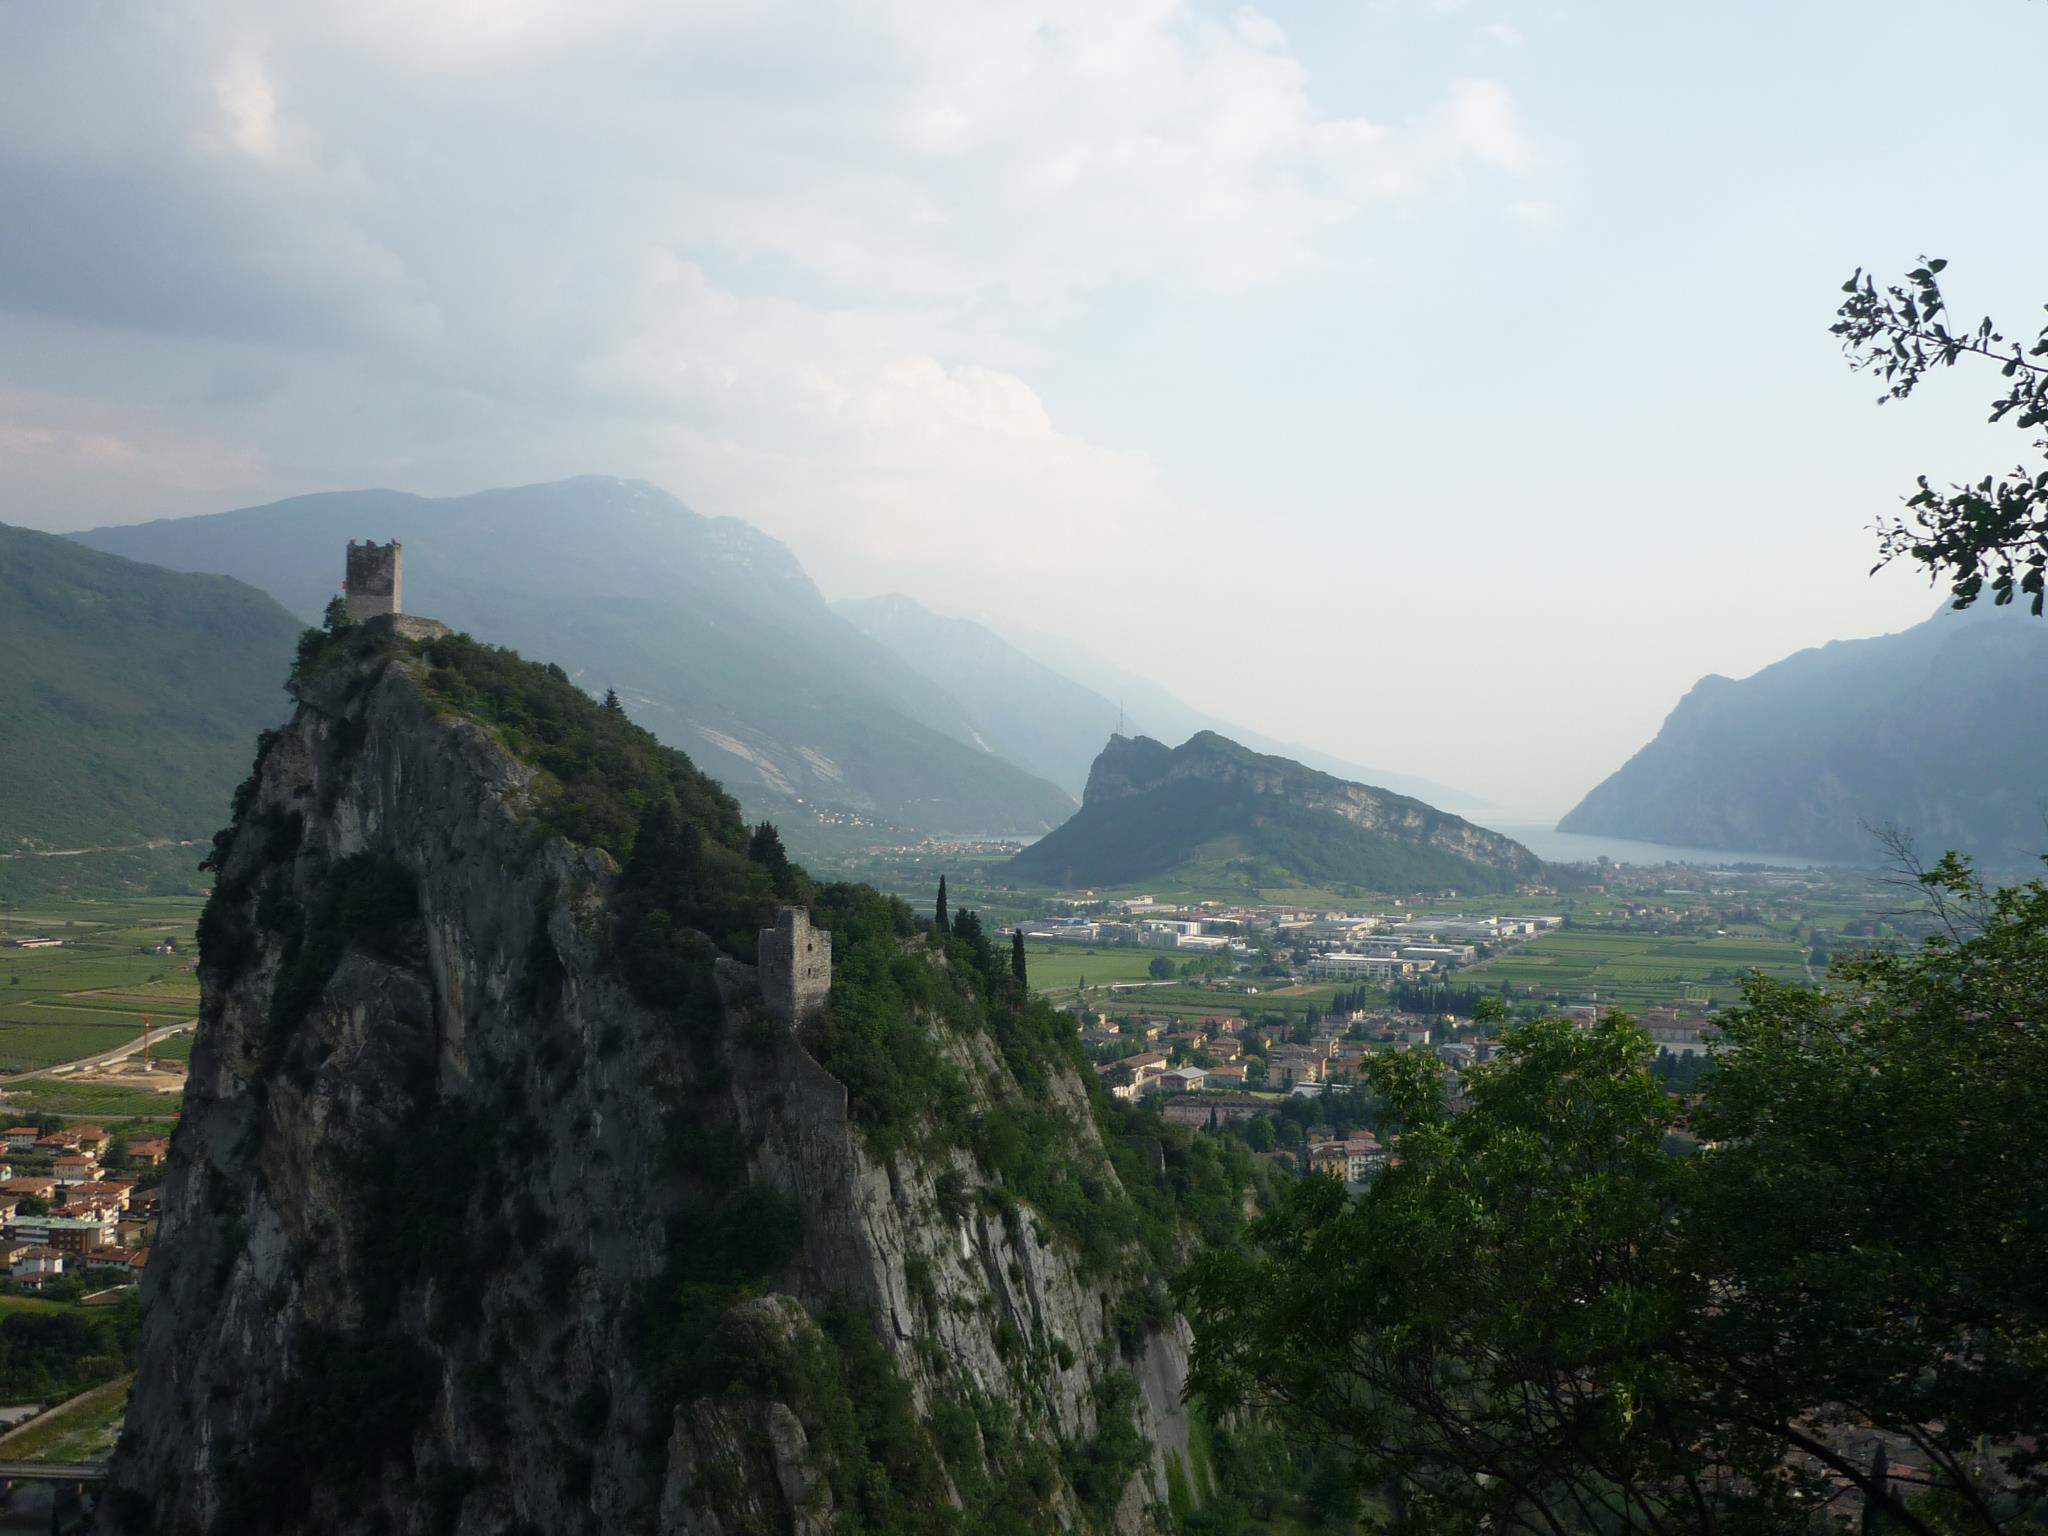
\includegraphics[width=0.9\linewidth,height=0.5\textheight]{antechima}
\hfill\captionof{figure}{Blick von der Antechima in das untere Sarchetal.}
\end{flushright}
\end{minipage}
\begin{minipage}[h]{.5\textwidth}
Wir dekomprimieren nach obigem Verfahren und setzen sämtliche rgb-Werte auf r$00$.
\begin{tabular}{c|c|c}
Symbol & Häufigkeit & Wahrscheinlichkeit
\\
\hline
33&	73876&	0.008806705474853516\\ \hline
34&	72291&	0.008617758750915527\\ \hline
35&	70384&	0.008390426635742188\\ \hline
36&	68368&	0.008150100708007812\\ \hline
37&	66323&	0.007906317710876465\\ \hline
38&	64607&	0.007701754570007324\\ \hline
39&	62227&	0.007418036460876465\\ \hline
40&	59856&	0.0071353912353515625\\ \hline
41&	57758&	0.0068852901458740234\\ \hline
42&	55613&	0.006629586219787598\\ \hline
43&	53136&	0.0063343048095703125\\ \hline
44&	50396&	0.006007671356201172\\ \hline
45&	48412&	0.005771160125732422\\ \hline
46&	45429&	0.005415558815002441\\ \hline
47&	43096&	0.005137443542480469\\ \hline
48&	41076&	0.004896640777587891\\ \hline
49&	38609&	0.004602551460266113\\ \hline
50&	36859&	0.004393935203552246\\ \hline
\end{tabular}
\end{minipage}
\hfill
\begin{minipage}[h]{.4\textwidth}
\begin{flushright}
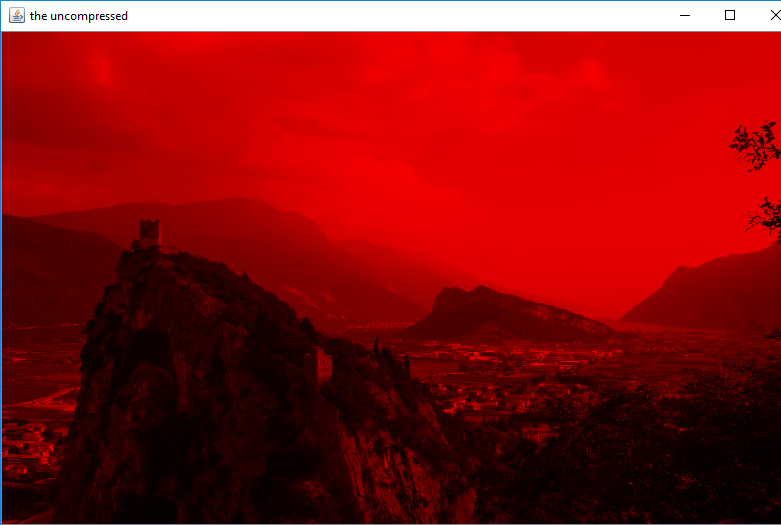
\includegraphics[width=0.9\linewidth,height=0.5\textheight]{uncompressed}
\end{flushright}
\end{minipage}
\captionof{figure}{Auszug: erste 50 Symbole - Fortsetzung}
\end{Beispiel}
\newpage
\section{Ergebnisse}
Im Folgenden wird der Einfluss der Normalisierung und der Filterung auf Bilder demonstriert.
Die Implementierung wurde in Java umgesetzt und steht unter \url{https://github.com/Hau-Bold/ImageProcessor} zu Verfügung.
\subsection{Ergebnisse der Normalisierung}
Im Folgenden wird der Einfluss der Normalisierung auf ein Bild (Siehe nächster Abschnitt Filtertyp 0) demonstriert:
\par
\hspace{1.5cm}
\begin{center}
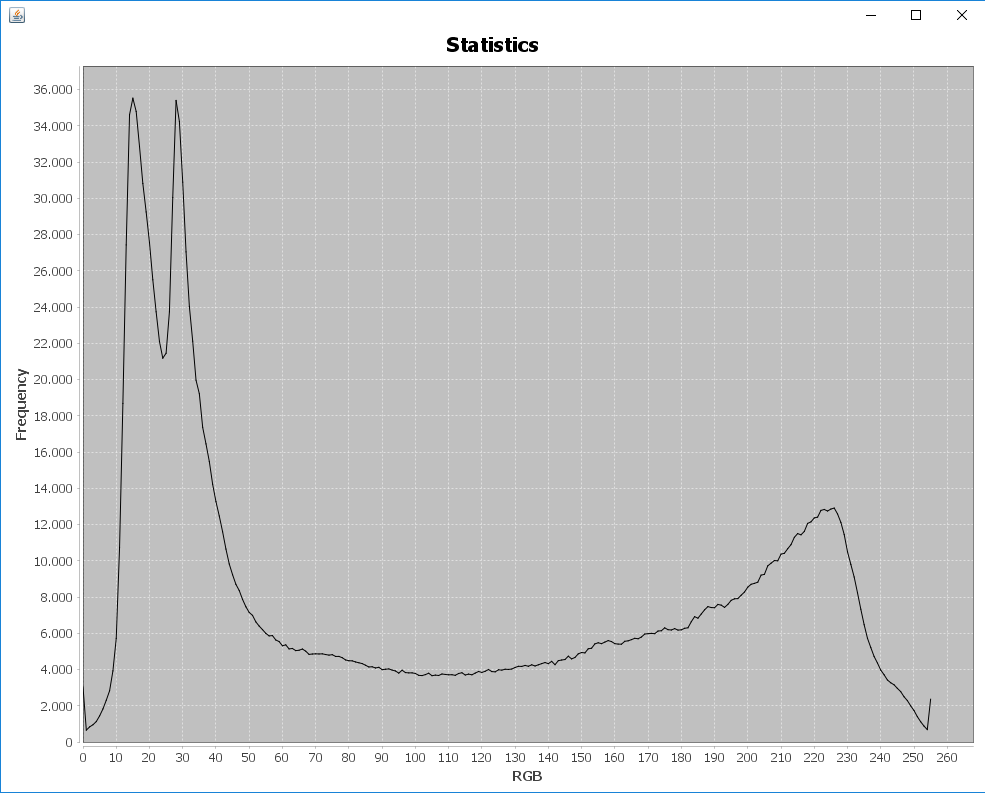
\includegraphics[width=0.8\linewidth,height=0.7\textheight]{Normalization/unnormalized}
\captionof{figure}{Häufigkeiten - Ohne Normalisierung}
\end{center}
\begin{center}
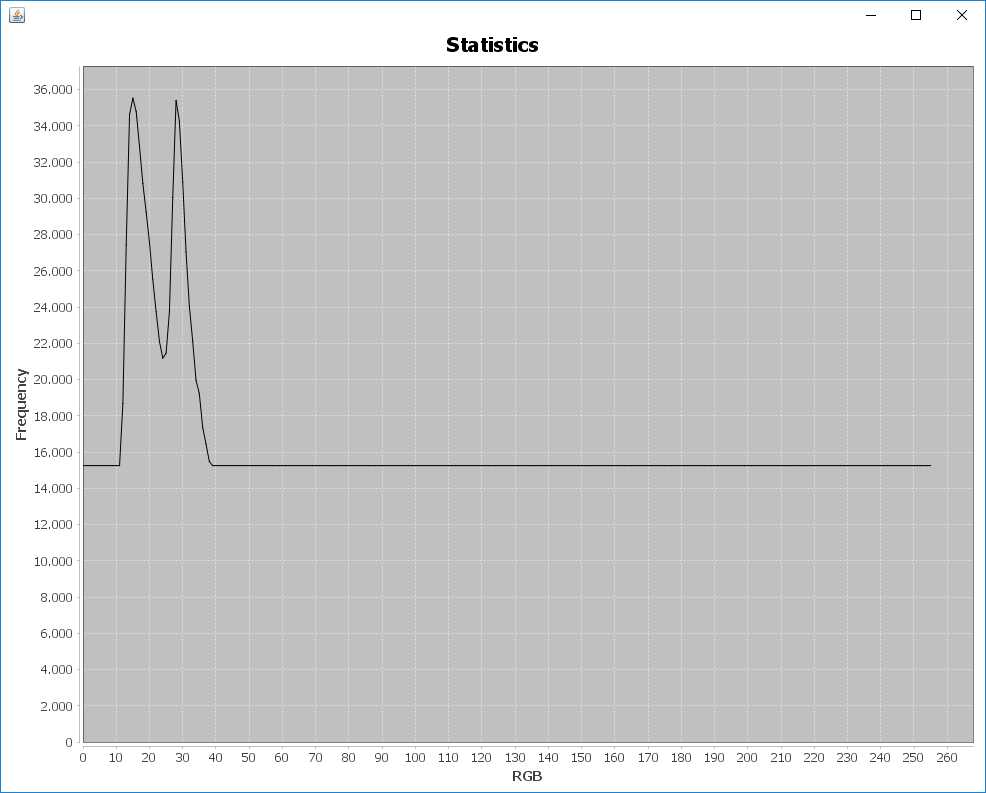
\includegraphics[width=0.8\linewidth,height=0.7\textheight]{Normalization/normalized}
\captionof{figure}{Häufigkeiten - Normalisierung {\tt{rans}}}
\end{center}
\begin{center}
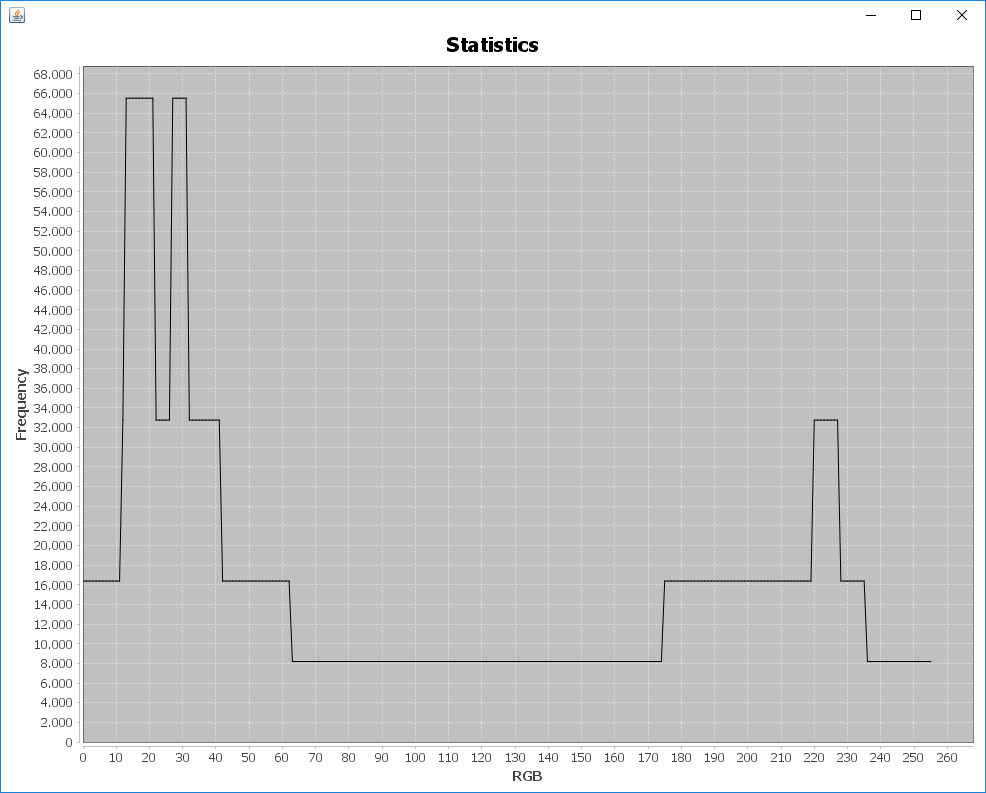
\includegraphics[width=0.8\linewidth,height=0.7\textheight]{Normalization/normalizedPowerOfTwo}
\captionof{figure}{Häufigkeiten - Normalisierung {\tt{uans}}}
\end{center}
\newpage
\subsection{Ergebnisse der Filterung}
Im Folgenden wird er Einfluss der verwendeten Filter demonstriert. 
\par
\hspace{1.5cm}
%\begin{center}
%\includegraphics[width=0.8\linewidth,height=0.7\textheight]{{\tt{pre}}conditioning/Bounty}
%\captionof{figure}{Filtertyp 0 - {\tt{none}}}
%\end{center}
%
%\begin{center}
%\includegraphics[width=0.8\linewidth,height=0.7\textheight]{{\tt{pre}}conditioning/test_SUB}
%\captionof{figure}{Filtertyp 1 - {\tt{sub}}}
%\end{center}
%
%\begin{center}
%\includegraphics[width=0.8\linewidth,height=0.7\textheight]{{\tt{pre}}conditioning/test_UP}
%\captionof{figure}{Filtertyp 2 - {\tt{up}}}
%\end{center}
%
%\begin{center}
%\includegraphics[width=0.8\linewidth,height=0.7\textheight]{{\tt{pre}}conditioning/test_AVERAGE2}
%\captionof{figure}{Filtertyp 3 - {\tt{average2}}}
%\end{center}
%
%\begin{center}
%\includegraphics[width=0.8\linewidth,height=0.7\textheight]{{\tt{pre}}conditioning/test_AVERAGE3}
%\captionof{figure}{Filtertyp 4 - {\tt{average3}}}
%\end{center}
%
%\begin{center}
%\includegraphics[width=0.8\linewidth,height=0.7\textheight]{{\tt{pre}}conditioning/test_AVERAGE4}
%\captionof{figure}{Filtertyp 5 - {\tt{average4}}}
%\end{center}
%
%\begin{center}
%\includegraphics[width=0.8\linewidth,height=0.7\textheight]{{\tt{pre}}conditioning/test_AVERAGE5}
%\captionof{figure}{Filtertyp 6 - {\tt{average5}}}
%\end{center}
%
%\begin{center}
%\includegraphics[width=0.8\linewidth,height=0.7\textheight]{{\tt{pre}}conditioning/test_AVERAGE6}
%\captionof{figure}{Filtertyp 7 - {\tt{average6}}}
%\end{center}\begin{center}
%
%\includegraphics[width=0.8\linewidth,height=0.7\textheight]{{\tt{pre}}conditioning/test_AVERAGE7}
%\captionof{figure}{Filtertyp 8 - {\tt{average7}}}
%\end{center}
%
%\begin{center}
%\includegraphics[width=0.8\linewidth,height=0.7\textheight]{{\tt{pre}}conditioning/test_AVERAGE8}
%\captionof{figure}{Filtertyp 9 - {\tt{average8}}}
%\end{center}

\begin{center}

\includegraphics[width=0.8\linewidth,height=0.7\textheight]{preconditioning/test_PAETH}
\captionof{figure}{Filtertyp 6 - {\tt{paeth}}}
\end{center}
\newpage
\subsubsection{Verhalten der Entropie unter Verwendung der Filterung und Normalisierung}
Abschließend geben wir das Verhalten der Entropie unter Verwendung der Normalisierung der Filterung wieder. Stufe 0 steht für die Entropie ohne Normalisierung, Stufe 1 für die Entropie nach Normalisierung. Stufe 2 (3) gibt den Wert der Entropie nach Verwendung eines Filters ohne (mit) vorheriger Normalisierung wieder,  und Stufe 4 (5) den Wert nach Einsatz eines Filters und anschließender Normalisierung mit (ohne) vorheriger Normalisierung. 
\par
Für die Normalisierung ANS erhält man folgende Werte:
\par
\vspace{1cm}
\begin{tabular}{c | c | c | c | c | c | c}
Filtertyp & 0 &  1 & 2 & 3 & 4A & 4B
\\
\hline
\textbf{{\tt{none}}} &  7.58792 & 7.58793 & 7.58792 & 7.58792  & 7.58793 &  7.58792
\\
\textbf{Sub} & 7.58792 &   7.58793 & 5.52772 &  5.52772 &5.52773  & 5.52773 
\\
\textbf{Up} & 7.58792 &  7.58793 & 5.3858 & 5.3858  & 5.38582 & 5.38582 
\\
\textbf{Average2} & 7.58792 &  7.58793 & 6.1528 & 6.1528 & 6.1528 & 6.1528 
\\
\textbf{Average3} & 7.58792 &  7.58793 & 6.39763 & 6.39763 & 6.39762 & 6.39762 
\\
\textbf{Average4} & 7.58792 &  7.58793 & 6.58027 & 6.58027 & 6.58027 & 6.58027 
\\
\textbf{Average5} & 7.58792 &  7.58793 & 6.95311 & 6.95311 & 6.95314 & 6.95314 
\\
\textbf{Average6} & 7.58792 &  7.58793 & 7.16235 & 7.16235 & 7.16235 &  7.16235 
\\
\textbf{Average7} & 7.58792 &  7.58793 & 7.2852 &  7.2852 &  7.2852 & 7.2852 
\\
\textbf{Average8} & 7.58792 &  7.58793 & 7.38257 & 7.38257  & 7.38258 & 7.38258 
\\
\textbf{Paeth} & 7.58792 &  7.58793 & 5.00477 &  5.00477  &  5.00478 & 5.00478 
\end{tabular}
\par
\vspace{1cm}

Für die Normalisierung uABS erhält man folgende Werte:
\par
\vspace{1cm}
\begin{tabular}{c | c | c | c | c | c | c}
Filtertyp & 0 &  1 & 2 & 3 & 4 & 5
\\
\hline
\textbf{{\tt{none}}} &  7.58792 & 7.63281 & 7.58792 & 7.58792  & 7.58793 &  7.63281
\\
\textbf{Sub} & 7.58792 &   7.63281 & 5.52772 &  5.52772 &  5.52773   & 6.0918
\\
\textbf{Up} & 7.58792 &  7.63281 & 5.3858 & 5.3858  &  5.38582  &  6.00684 
\\
\textbf{Average2} & 7.58792 &  7.63281 & 6.1528 & 6.1528 & 6.1528  & 6.20898
\\
\textbf{Average3} & 7.58792 &  7.63281 & 6.39763 & 6.39763 & 6.1528 & 6.6543 
\\
\textbf{Average4} & 7.58792 &  7.63281 & 6.58027 & 6.58027 & 6.58027  & 6.62695 
\\
\textbf{Average5} & 7.58792 &  7.63281 & 6.95311 & 6.95311 & 7.10156 &  7.10156 
\\
\textbf{Average6} & 7.58792 &  7.63281 & 7.16235 & 7.16235 & 7.23828 &  7.23828 
\\
\textbf{Average7} & 7.58792 &  7.63281 & 7.2852 &  7.2852 & 7.47656   &  7.47656
\\
\textbf{Average8} & 7.58792 &  7.63281 & 7.38257 &  7.38257  & 7.50391  & 7.50391
\\
\textbf{Paeth} & 7.58792 &  7.63281 & 5.00477 &   5.00477  & 5.21973  & 5.21973 
\end{tabular}


\newpage
\section{Abbildungsverzeichnis}
\listoffigures

\newpage
\section{Kommandozeilenparameter}\label{Kommandozeilenparameter}
\newpage
\listoffigures
\newpage
\section{Literaturverzeichnis}
\thispagestyle{plain}
\begin{thebibliography}{DiplRS}
\bibitem[1]{Krajcevski} Krajcevski P., Pratapa S., Manocha D. {\it GST: GPU-decodable Supercompressed Textures},  Proc. of ACM SIGGRAPH Asia, (2016).
\bibitem[2]{Giesen}  Giesen F. {\it Interleaved entropy coders},  arXiv:1402.3392 , (2014).
\bibitem[3]{Duda}  Duda J. {\it Asymmetric numeral systems: entropy coding combining speed of Huffman coding with compression rate of arithmetic coding},  CoRR, abs/1311.2540v2, (2014).
\bibitem[4]{henne} Li\'{s}kiewicz M., Fernau H. {\it Datenkompression} 
\url{ https://www.uni-trier.de/fileadmin/fb4/prof/INF/TIN/Folien/DK/script.pd}.
\bibitem[5]{Li}  Li M.,  Vit\'{a}nyi P.{\it An introduction to Kolmogorov complexity and its applications}, 2. Auflage, Springer, (1997).
\bibitem[6]{Lajmi} Lajmi L. {\it Informationstheorie und Codierung}
\url{https://www.ostfalia.de/export/sites/default/de/pws/lajmi/Lehre/Codierungstheorie/pdf/Quellencodierung_SS15.pdf}.
\bibitem[7]{Rohling} Rohling H. {\it Einführung in die Informations- und Codierungstheorie} B.G. Teubner Stuttgart, (1995).
\bibitem[8]{Huffman} Huffman D. A. {\it A method for the construction of minimum-redundancy codes} Proceedings of the I.R.E.., S. 1098-1101, (1952).
\bibitem[9]{fb} {\it Smaller and faster data compression with Zstandard} \url{https://code.facebook.com/{\tt{post}}s/1658392934479273/smaller-and-faster-data-com{\tt{pre}}ssion-with-zstandard/}
\bibitem[10]{apple}{\it Apple Open-Sources its New Compression Algorithm LZFSE} \url{https://www.infoq.com/news/2016/07/apple-lzfse-lossless-opensource}
\bibitem[11]{google}{\it Google Draco 3D compressor} \url{https://github.com/google/draco}
\bibitem[12]{png}{\it PNG (Portable Network Graphics) Specification} \url{https://www.w3.org/TR/PNG-Filters.html}
\bibitem[13]{Breymann}{Breymann U.} {\it DER C++ Programmierer},Carl Hanser Verlag München, (2015).
\bibitem[14]{Breymann}{Williams A.} {\it C++ Concurrency IN ACTION},Manning Publications Co Shelter Island NY 11964 (2012).
\end{thebibliography}

\newpage
\begin{titlepage}
\section*{Erklärung:}
\noindent {\large Die vorliegende Bachelorarbeit wurde am Institut für Informatik  der Hochschule Coburg nach einem Thema von Herrn Prof.~Dr.~Quirin~Meyer erstellt.
\newline Hiermit versichere ich, dass ich diese Arbeit selbstständig angefertigt und dazu nur die angegebenen Quellen verwendet habe.

\vspace{1.5cm}

\noindent Coburg, den \today

\vspace{0.5cm}

\raggedleft Michael Krasser\quad\quad \par}

\vfill
\end{titlepage}

\end{document}
